\documentclass[11pt]{article}
\usepackage[margin=1.1in]{geometry}
\usepackage{amsmath,amssymb,amsthm}
\usepackage{tikz}
\usepackage[colorlinks=true,linkcolor=blue,citecolor=blue,urlcolor=blue,
  pdftitle={Exact two-colour Rado numbers of x1+ax2-x3=c},
  pdfauthor={Jan Sherzad Colet},
  pdfkeywords={Rado numbers, Ramsey theory on the integers, monochromatic
    solutions, SAT solving, DRAT certificates}]{hyperref}

\newtheorem{theorem}{Theorem}
\newtheorem{lemma}{Lemma}[section]
\theoremstyle{remark}
\newtheorem{remark}{Remark}
\theoremstyle{definition}
\newtheorem{example}[theorem]{Example}

\newcommand{\Rad}{\mathrm{Rad}_2}
\newcommand{\vtwo}{\nu_2}
\DeclareMathOperator{\lcm}{lcm}

\title{Exact two-colour Rado numbers of $x_1 + a x_2 - x_3 = c$: \\
the window $0 < c < a$ and two conjectures \\ of Dwivedi and Tripathi}
\author{Jan Sherzad Colet\thanks{Independent researcher.
\texttt{jansherzadcolet@gmail.com}. Every computational
claim in this note is accompanied by machine-checkable certificates (witness
colourings and DRAT proofs verified by \texttt{drat-trim}); the complete
verification package is available from the author and at
\url{https://github.com/4Gatitos/RadoNumbers}.}}
\date{July 2026}

\begin{document}
\maketitle

\begin{abstract}
For integers $a \ge 1$ and $c$, the $2$-colour Rado number $\Rad(a;c)$ is the
least $N$ such that every $2$-colouring of $\{1,\dots,N\}$ admits a
monochromatic solution of $x_1 + a x_2 - x_3 = c$, repeated values being
allowed; it exists if and only if $\vtwo(a) \le \vtwo(c)$, where $\vtwo$ is
the $2$-adic valuation. Dwivedi and Tripathi
[\emph{Integers} \textbf{20} (2020), \#A36] determined $\Rad(a;c)$ in several
parameter ranges and asked for the remaining exact values. We resolve the
window $0 < c < a$ completely: writing $d = a-c$ and $r \equiv a \pmod{2d}$
with $r \in [1,2d]$,
\[
\Rad(a;\,a-d) \;=\;
\begin{cases}
2a+2, & d = 1,\\[2pt]
(a+3)d + a - \min(r-1,\, d-1), & d \ge 2,
\end{cases}
\]
whenever the number exists. The upper-bound argument extends to $c \le 0$,
proving Conjecture~1 of Dwivedi and Tripathi in full; their Conjecture~2
then follows by a reflection argument. In every regime the final obstruction
is precisely the $2$-adic existence condition. In the remaining band
$a < c < a(K+2)$, where
$K+1 = \lceil (1+c(a+3))/(1+a(a+3)) \rceil$ is the general lower bound of
Dwivedi and Tripathi, the values appear to follow no closed formula; there
we prove an extension of their multiples theorem and announce the complete
determination of the band, with proofs to appear in a companion manuscript.
All results are corroborated by more than $30{,}000$ SAT-computed values
with independently verifiable certificates.

\medskip
\noindent\emph{2020 Mathematics Subject Classification:} 05D10 (primary);
11B75, 68R05 (secondary).

\noindent\emph{Keywords:} Rado numbers, Ramsey theory on the integers,
monochromatic solutions, SAT solving, DRAT certificates.
\end{abstract}

\section{Introduction}

For an equation $\mathcal{E}$ in the variables $x_1,\dots,x_m$, the
$2$-colour Rado number $\Rad(\mathcal{E})$ is the least positive integer $N$
such that every $2$-colouring of the integer interval $[1,N]$ contains a
monochromatic solution of $\mathcal{E}$, that is, a solution all of whose
entries receive the same colour; solutions with repeated values are allowed.
Following Dwivedi and Tripathi \cite{DT2020}, we study the family
\[
\mathcal{E}_{a,c}\colon\quad x_1 + a x_2 - x_3 = c ,
\]
where $a$ is a positive integer and $c$ any integer, and write
$\Rad(a;c) := \Rad(\mathcal{E}_{a,c})$.

Dwivedi and Tripathi proved that $\Rad(a;c)$ exists if and only if
$\vtwo(a) \le \vtwo(c)$ (with $\vtwo(0) = \infty$), and determined it exactly
in several parameter ranges: for $c \le 0$ when $a \mid c$, or when $a$ is odd
and $c$ is sufficiently negative (in a precise residue-dependent sense); for
$c = ma$ with $1 < m \le a+1$; and for $c > a$ sufficiently large. In the
remaining ranges they gave upper and lower bounds, together with two
conjectures for the zones adjacent to their theorems. In the recent paper
\cite{DT2025} the same authors returned to the problem and wrote that
``it would be desirable to determine the exact value of the Rado number in
all cases.''

In the window $0 < c < a$ their results give the bounds
$(a+3)(a-c)+1 \le \Rad(a;c) \le (2a+1)(a-c)+1$ (for odd $a$; similarly for
even $a$), and no conjecture. A subsequent paper of Arora, Dwivedi and
Tripathi \cite{ADT2025} extends the lower bound to a general class of
equations $\sum_i a_i x_i - x_m = c$, with matching exact values when the
coefficient multiset is \emph{$2$-distributable}; for the equation studied
here the multiset is $\{1, a\}$, which is $2$-distributable only for
$a \le 2$, so in our window that paper again yields exactly the lower bound
$(a+3)(a-c)+1$. This note closes the window completely --- in particular,
the lower bound of \cite{DT2020,ADT2025} is never tight there for
$a \ge 3$, $d \ge 2$.

\begin{theorem}\label{thm:d1}
Let $a \ge 3$ be odd. Then $\Rad(a;\,a-1) = 2a+2$.
\end{theorem}

(For even $a$ the number $\Rad(a;a-1)$ does not exist, since $a-1$ is odd;
so Theorem~\ref{thm:d1} covers the whole diagonal $c = a-1$. The case $a=3$,
i.e.\ $\Rad(3;2) = 8$, appears in \cite{DT2020}; the general statement is
new.)

\begin{theorem}\label{thm:main}
Let $a > d \ge 2$ with $\vtwo(a) \le \vtwo(a-d)$, and write $a = 2dq + r$
with $q \ge 0$ an integer and $r \in [1, 2d]$. Then
\[
\Rad(a;\,a-d) \;=\; (a+3)d + a - \min(r-1,\, d-1).
\]
\end{theorem}

Under the existence condition one automatically has $r \in [1, 2d-1]$
(Lemma~\ref{lem:norm}), and the two theorems together determine
$\Rad(a;c)$ for every pair with $0 < c < a$ for which it exists. It is
curious that the uniform formula of Theorem~\ref{thm:main} fails for $d = 1$
by exactly one unit: the extremal colouring family of
Section~\ref{sec:family} degenerates at $d=1$ into a colouring of
$[1, 2a+2]$ which is \emph{not} valid --- and the proof of
Theorem~\ref{thm:d1} shows that nothing else works at that length either.

Our third and fourth results settle the two conjectures of \cite{DT2020}.
For $c \le 0$ one has $d = a - c \ge a$, so that $r \equiv a \pmod{2d}$ is
simply $r = a$: the window formula of Theorem~\ref{thm:main} formally
reduces to $(a+3)d + a - (a-1) = (a+3)(a-c) + 1$, which is exactly the value
predicted by Conjecture~1 of \cite{DT2020}. This is no coincidence: our
upper-bound proof for the regime $r \le d$ extends to this degenerate case
($q = 0$ in the normalisation $a = 2dq + r$) after adjusting two range
conditions, and the lower bound is Theorem~2 of \cite{DT2020}.

\medskip
\noindent\textbf{Theorem~\ref{thm:c1}} (Conjecture~1 of \cite{DT2020}).
\emph{Let $a \ge 1$ and $c \le 0$ with $\vtwo(a) \le \vtwo(c)$. Then
$\Rad(a;c) = (a+3)(a-c) + 1$.}

\medskip
\noindent\textbf{Theorem~\ref{thm:c2}} (Conjecture~2 of \cite{DT2020}).
\emph{Let $a \ge 1$ and let $c \ge a(K+2)$ with $\vtwo(a) \le \vtwo(c)$, where
$K = \bigl\lceil (1 + c(a+3)) / (1 + a(a+3)) \bigr\rceil - 1$. Then
$\Rad(a;c) = K + 1$.}

\medskip
Theorem~\ref{thm:c2} follows from Theorem~\ref{thm:c1} by a
reflection argument generalising the proof of Theorem~7 of \cite{DT2020}
(Section~\ref{sec:conj}). Taken together, these results determine
$\Rad(a;c)$ exactly for every $c \le 0$, every $0 < c \le a$, and every
$c \ge a(K+2)$. The remaining zone --- the band $a < c < a(K+2)$ --- behaves
very differently: no closed formula holds there, the fluctuations being of
Sturmian type. Section~\ref{sec:band} states what we can prove about the
band: an extension of the multiples theorem of \cite{DT2020}
(Theorem~\ref{thm:band-mult}, proved here), the complete determination of
the band's deep tail, where the threshold is itself a Rado number from the
window $0 < c < a$ (Theorem~\ref{thm:band-tail}), and the exact
determination of the whole band by a polynomial-time algorithm
(Theorem~\ref{thm:band-alg}); the proofs of the last two will appear in the
companion manuscript \cite{companion}.

Table~\ref{tab:summary} and Figure~\ref{fig:zones} summarise the resulting
picture.

\begin{table}[ht]
\centering
\begin{tabular}{lll}
\hline
zone & $\Rad(a;c)$ & reference \\
\hline
$c \le 0$ & $(a+3)(a-c)+1$ & Theorem~\ref{thm:c1} \\
$0 < c < a$, $d = 1$ & $2a+2$ & Theorem~\ref{thm:d1} \\
$0 < c < a$, $d \ge 2$ & $(a+3)d + a - \min(r-1,d-1)$ & Theorem~\ref{thm:main} \\
$c = a$ & $1$ & \cite{DT2020} \\
$a < c < a(K+2)$, $a \mid c$ & $c/a$ & Theorem~\ref{thm:band-mult} \\
$a < c < a(K+2)$, $a \nmid c$ & deep-tail formula; exact algorithm &
Theorems~\ref{thm:band-tail}--\ref{thm:band-alg}$^{*}$ \\
$c \ge a(K+2)$ & $K+1$ & Theorem~\ref{thm:c2} \\
\hline
\end{tabular}
\caption{The value of $\Rad(a;c)$ on each parameter zone, assuming the
existence condition $\vtwo(a) \le \vtwo(c)$. Here $d = a-c$,
$r \equiv a \pmod{2d}$ with $r \in [1,2d]$, and
$K = \lceil (1+c(a+3))/(1+a(a+3)) \rceil - 1$. Entries marked $^{*}$ are
announced here and proved in the companion manuscript; all other entries
are proved in this note or in \cite{DT2020}.}
\label{tab:summary}
\end{table}

\begin{figure}[ht]
\centering
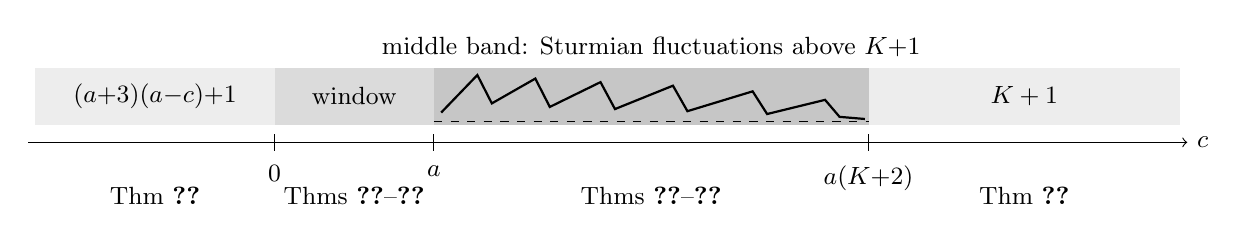
\begin{tikzpicture}[xscale=0.92, yscale=0.9, font=\small]
% axis
\draw[->] (-3.4,0) -- (12.6,0) node[right] {$c$};
% zone boundaries
\foreach \x/\lab in {0/{$0$}, 2.2/{$a$}, 8.2/{$a(K{+}2)$}}
  \draw (\x,-0.12) -- (\x,0.12) node[below=8pt] {\lab};
% zone bands
\fill[gray!14] (-3.3,0.25) rectangle (0,1.05);
\fill[gray!28] (0,0.25) rectangle (2.2,1.05);
\fill[gray!45] (2.2,0.25) rectangle (8.2,1.05);
\fill[gray!14] (8.2,0.25) rectangle (12.5,1.05);
% zone labels (formulas)
\node at (-1.65,0.65) {$(a{+}3)(a{-}c){+}1$};
\node at (1.1,0.65) {window};
\node at (5.2,1.35) {middle band: Sturmian fluctuations above $K{+}1$};
\node at (10.35,0.65) {$K+1$};
% theorem tags
\node at (-1.65,-0.75) {Thm~\ref{thm:c1}};
\node at (1.1,-0.75) {Thms~\ref{thm:d1}--\ref{thm:main}};
\node at (5.2,-0.75) {Thms~\ref{thm:band-mult}--\ref{thm:band-alg}};
\node at (10.35,-0.75) {Thm~\ref{thm:c2}};
% sawtooth inside the band, above the K+1 baseline
\draw[thick] (2.3,0.42) -- (2.8,0.95) -- (3.0,0.55) -- (3.6,0.9) -- (3.8,0.5)
  -- (4.5,0.85) -- (4.7,0.47) -- (5.5,0.8) -- (5.7,0.44) -- (6.6,0.72)
  -- (6.8,0.4) -- (7.6,0.6) -- (7.8,0.36) -- (8.15,0.33);
\draw[dashed] (2.2,0.3) -- (8.2,0.3);
\end{tikzpicture}
\caption{The zones of $\Rad(a;c)$ (schematic, $c$ increasing to the right).
Outside the middle band the value follows the closed formulas of
Table~\ref{tab:summary}; inside it, the value oscillates above the lower
bound $K+1$ of \cite{DT2020} (dashed) in a quasi-periodic, three-distance
pattern, and is determined by the algorithm of Theorem~\ref{thm:band-alg}.}
\label{fig:zones}
\end{figure}

The proofs have a common architecture, which generalises the forcing
arguments of \cite{DT2020}. The lower bounds are witnessed by an explicit
two-parameter family of periodic colourings with regularly spaced phase
defects (Section~\ref{sec:family}). The upper bounds are rigidity arguments:
any putative valid colouring of the critical interval is forced, triple by
triple, into a highly structured pattern, and the final obstruction that
kills the pattern is, in both parameter regimes, \emph{exactly} the $2$-adic
existence condition $\vtwo(a) \le \vtwo(a-d)$ --- in the regime $r \le d$
through the fact that $\gcd(r, 2d) \mid d$, and in the regime $r > d$
through the incompatibility of antipodal and $s$-antiperiodic patterns on
$\mathbb{Z}_{2d}$ when $\vtwo(s) \ne \vtwo(d)$, $s = r-d$
(Sections~\ref{sec:ub1} and~\ref{sec:ub2}).

\paragraph{Methodology and verifiability.}
The formula of Theorem~\ref{thm:main}, the extremal family, and the key
structural lemmas were first \emph{discovered} through an extensive
SAT-solver-based computation of exact Rado numbers: $3662$ pairs $(a,c)$
with $3 \le a \le 15$, $-100 \le c \le 300$, later extended along $0 < c < a$
up to $a = 45$. Every computed value $\Rad(a;c) = N$ is certified in both
directions: a valid colouring of $[1,N-1]$ (checkable by a trivial
independent program) and a DRAT proof of unsatisfiability at $N$, generated
by CaDiCaL~2.1.3 \cite{cadical} and verified by \texttt{drat-trim} against an independently
regenerated CNF encoding. The proofs presented here are, however, entirely
self-contained and human-readable; the computations play no logical role in
the theorems of this note: they served to discover the statements and to
corroborate them independently. Every one of the $925$ computed values with
$c \le 0$, and every value in the ranges of the four theorems, matches the
formulas proved here (Section~\ref{sec:comp}).

\section{Preliminaries}\label{sec:prelim}

Throughout, $[u,v]$ denotes $\{u, u+1, \dots, v\}$ and $\vtwo$ the $2$-adic
valuation. A \emph{colouring} is a map $\chi\colon [1,N] \to \{0,1\}$; it is
\emph{valid} (for the pair $(a,c)$) if no solution
$(x_1,x_2,x_3) \in [1,N]^3$ of $x_1 + a x_2 - x_3 = c$ is monochromatic.

Solving for $x_3$, we see that the solutions in $[1,N]^3$ are exactly the
triples
\begin{equation}\label{eq:triples}
T(x,k) \;=\; \bigl(x,\; k,\; x + a(k-1) + d\bigr), \qquad d := a - c,
\end{equation}
with $x, k \in [1,N]$ and $1 \le x + a(k-1) + d \le N$ (for $d \ge 1$, which
holds everywhere outside Section~\ref{sec:band}, the constraint
$x + a(k-1) + d \ge 1$ is automatic). We record two standard facts.

\begin{lemma}[monotonicity]\label{lem:mono}
If $[1,N]$ admits a valid colouring, so does $[1,N']$ for every $N' \le N$
(restrict the colouring). Hence $\Rad(a;c) > N$ if and only if $[1,N]$
admits a valid colouring, and to determine $\Rad(a;c) = N$ it suffices to
exhibit a valid colouring of $[1,N-1]$ and to prove that no valid colouring
of $[1,N]$ exists.
\end{lemma}

\begin{lemma}[colour symmetry]\label{lem:wlog}
$\chi$ is valid if and only if $1-\chi$ is valid. In any proof by
contradiction we may therefore normalise $\chi(1) = 0$.
\end{lemma}

\begin{lemma}[normalisation]\label{lem:norm}
Let $d \ge 1$, $a > d$, and write $a = 2dq + r$ with $r \in [1, 2d]$.
\begin{enumerate}
\item[(i)] If $r = 2d$, then $\vtwo(a) > \vtwo(a-d)$, so $\Rad(a;a-d)$ does
not exist. Under the existence condition, therefore, $r \in [1, 2d-1]$.
\item[(ii)] If $r \le d$ then $q \ge 1$ (so $a \ge 2d+1$).
\item[(iii)] If $r = d + s$ with $s \in [1, d-1]$, then $q \ge 0$, and the
existence condition is equivalent to $\vtwo(s) \ne \vtwo(d)$
(Lemma~\ref{lem:2adic-b} below); if $r \le d$, the existence condition
implies $\vtwo(r) \le \vtwo(d)$, hence $\gcd(r,2d) \mid d$
(Lemma~\ref{lem:2adic-a} below).
\end{enumerate}
\end{lemma}

\begin{proof}
(i) Write $a = 2dm$, $m \ge 1$. Then $\vtwo(a) \ge \vtwo(d)+1$ while
$a - d = d(2m-1)$ gives $\vtwo(a-d) = \vtwo(d)$.
(ii) If $q = 0$ then $a = r \le d$, contradicting $a > d$.
(iii) The two $2$-adic statements are proved as
Lemmas~\ref{lem:2adic-a} and~\ref{lem:2adic-b} in the sections where they
are used.
\end{proof}

\section{The diagonal $c = a-1$: proof of Theorem~\ref{thm:d1}}\label{sec:d1}

Here $d = 1$ and the solution triples \eqref{eq:triples} are
$T(x,k) = (x, k, x + a(k-1) + 1)$.

\subsection*{Lower bound}
Colour $[1, 2a+1]$ by the classes
\[
A \;=\; \{\,x \text{ odd} : x \le a\,\} \cup \{\,x \text{ even} : a+3 \le x \le 2a\,\},
\qquad
B \;=\; [1, 2a+1] \setminus A .
\]
If a triple $T(x,k)$ lies in $[1, 2a+1]^3$ then $a(k-1) \le 2a-1$, so
$k \in \{1,2\}$. A monochromatic triple in $A$ would need $k = 1$ (as
$2 \notin A$: the even elements of $A$ start at $a+3$); but for $x \in A$ odd,
$x+1$ is even and $\le a+1$, hence in $B$, and for $x \in A$ even,
$x+1$ is odd and $\ge a+4$, hence in $B$. A monochromatic triple in $B$ would
need $k = 2$ (as $1 \notin B$); but for $x \in B$ even, $x \le a+1$: if
$x \le a-1$ then $x_3 = x + a + 1$ is even in $[a+3, 2a]$, hence in $A$,
and if $x = a+1$ then $x_3 = 2a+2$ is out of range; for $x \in B$ odd,
$x \ge a+2$, so $x_3 \ge 2a+3$ is out of range. Hence the colouring is valid
and $\Rad(a; a-1) \ge 2a+2$.

\subsection*{Upper bound}
Let $\chi$ colour $[1, 2a+2]$ with no monochromatic triple; by
Lemma~\ref{lem:wlog}, $\chi(1) = 0$.

\emph{Step 1.} $T(x,1) = (x,1,x+1)$ is a solution for every $x \le 2a+1$.
Since $\chi(1) = 0$, no two consecutive integers are both coloured $0$.
In particular $T(1,1) = (1,1,2)$ forces $\chi(2) = 1$.

\emph{Step 2.} $T(x,2) = (x,2,x+a+1)$ is a solution for $x \le a+1$. Since
$\chi(2) = 1$: if $\chi(x) = 1$ with $x \le a+1$, then $\chi(x+a+1) = 0$.

\emph{Step 3.} The pairs $\{x, x+a+1\}$, $x \in [1, a+1]$, partition
$[1, 2a+2]$. By Step~2 each pair contains a $0$, so $\#\chi^{-1}(0) \ge a+1$;
by Step~1, $\#\chi^{-1}(0) \le a+1$. Hence exactly $a+1$ zeros, no two
adjacent, in an interval of length $2a+2$: the zero set must be
\[
Z_j \;=\; \{1, 3, \dots, 2j-3\} \cup \{2j, 2j+2, \dots, 2a+2\}
\]
for some $j$, and $\chi(1) = 0$ forces $j \in [2, a+2]$.

\emph{Step 4.} Each $j$ is contradictory.
If $j = a+2$ (zeros are all the odds), the triple $(a+1, 2, 2a+2)$ is
monochromatic of colour $1$ ($a+1$ and $2a+2$ are even).
If $3 \le j \le a+1$, then $\chi(1) = \chi(3) = 0$ and $2a+2 \ge 2j$ is an
even member of $Z_j$; the triple $(1, 3, 2a+2)$ is monochromatic of colour
$0$.
If $j = 2$ (zeros are $\{1\} \cup \{4, 6, \dots, 2a+2\}$), then
$\chi(3) = \chi(2) = 1$ and $a+4$ is odd and $\ge 5$, hence coloured $1$;
the triple $(3, 2, a+4)$ is monochromatic of colour $1$ (note
$a + 4 \le 2a+2$ for $a \ge 2$). \qed

\section{The extremal family and the lower bound for $d \ge 2$}\label{sec:family}
% sec_lb.tex --- the extremal family colouring and the lower bound for d >= 2.
% This file is \input into Section 4 of the paper. It relies on the host results
% \eqref{eq:triples} (solution parametrisation), Lemma~\ref{lem:norm} (normalisation),
% Lemma~\ref{lem:wlog} (colour swap) and Lemma~\ref{lem:mono} (monotonicity).

Throughout this section fix $d \ge 2$ and $a \ge d+1$ with $\vtwo(a) \le \vtwo(a-d)$,
and write $a = 2dq + r$ with $q \ge 0$ and $r \in [1, 2d-1]$, as provided by
Lemma~\ref{lem:norm}. We distinguish two regimes. In \emph{regime 1} we have
$r \le d$; then $q \ge 1$, since $q = 0$ would give $a = r \le d$, contradicting
$a \ge d+1$; in particular $a \ge 2d+1$ in regime 1. In \emph{regime 2} we have
$r \ge d+1$; we set $s = r - d \in [1, d-1]$, and here $q \ge 0$, the value $q = 0$
occurring precisely when $d+1 \le a \le 2d-1$. Throughout we set
\[
  t = \max(d,\, 2d-r), \qquad N^{*} = (a+3)d + a - \min(r-1,\, d-1) - 1,
\]
so that $t = 2d-r \in [d, 2d-1]$ and $N^{*} = (a+3)d + a - r$ in regime 1, while
$t = d$ and $N^{*} = (a+2)d + a$ in regime 2 (as $\min(r-1, d-1)$ equals $r-1$ for
$r \le d$ and $d-1$ for $r \ge d+1$). Recall from \eqref{eq:triples} that the
solutions of $x_1 + a x_2 - x_3 = a - d$ with all values in $[1, N]$ are exactly
the triples $(x, k, y)$ with $y = x + a(k-1) + d$ and $x, k, y \in [1, N]$. We
shall exhibit a $2$-colouring $\chi$ of $[1, N^{*}]$ admitting no monochromatic
such triple. The colouring is defined by an explicit run-length list
(Lemma~\ref{lem:lb-family}) and then rewritten in a \emph{chunk--offset normal
form} $\chi(x) = \alpha(w(x)-1)$ (Lemma~\ref{lem:lb-normalform}); for every
in-range triple the offset increment obeys a trichotomy
(Lemma~\ref{lem:lb-trichotomy}), forcing in particular $k \le d+2$, and each of
the three resulting cases leads to a colour conflict (Theorem~\ref{thm:lb}). The
analysis is uniform in $q \ge 1$ (regime 1), respectively $q \ge 0$ (regime 2),
and covers the edge values $r = 1$, $r = d$, $r = d+1$, $r = 2d-1$ and $a = d+1$.

\begin{lemma}[the extremal family colouring]\label{lem:lb-family}
Keep the notation above, with $r \in [1, 2d-1]$. Let $\chi$ be the colouring of an
initial interval of the positive integers obtained by concatenating runs of
constant colour, the colours alternating and the first run having colour $1$ (so the
run of index $j$ has colour $1$ if $j$ is odd and colour $0$ if $j$ is even), with
run-length sequence
\begin{align*}
  \text{regime 1 } (r \le d)\colon &\quad
    [d]^{2q+1}\;\bigl([d+r]\,[d]^{2q-1}\bigr)^{d-1}\;[d+r]\,[d]^{2q+1};\\
  \text{regime 2 } (r > d,\ s = r-d)\colon &\quad
    [d]^{2q+2}\,[s]\;\bigl([d]^{2q+1}\,[s]\bigr)^{d-1}\;[d]^{2q+2}\,[s],
\end{align*}
where $[\ell]^{m}$ abbreviates $m$ consecutive runs of length $\ell$ and
$[\ell] = [\ell]^{1}$. Then:
(a) every run length is at least $1$;
(b) the total length equals $N^{*}$, so that $\chi \colon [1, N^{*}] \to \{0,1\}$;
(c) in regime 1 the $i$-th long $(d+r)$-run has run index $2qi + 2$, which is
even, hence colour $0$; in regime 2 every $s$-run except the last has odd index,
hence colour $1$, while the final $s$-run has even index, hence colour $0$.
\end{lemma}

\begin{proof}
(a) In regime 1: $d \ge 2$, $d + r \ge 3$, and $2q - 1 \ge 1$ because $q \ge 1$;
the multiplicities $2q+1$, $2q-1$ are positive. In regime 2: $d \ge 2$,
$s \in [1, d-1]$, and $2q+1 \ge 1$, $2q+2 \ge 2$ for $q \ge 0$.

(b) Regime 1: using $2dq = a - r$, the total length is
\[
  2\,d(2q+1) + d(d+r) + (d-1)\,d(2q-1)
  = (4dq + 2d) + (d^{2} + dr) + (2qd^{2} - d^{2} - 2qd + d)
  = 2qd^{2} + dr + 3d + 2dq,
\]
while
$N^{*} = (a+3)d + a - r = (2dq + r + 3)d + 2dq = 2qd^{2} + rd + 3d + 2dq$; the two
agree. Regime 2: using $2dq = a - d - s$ we have $d(2q+2) = a + d - s$ and
$d(2q+1) = a - s$, so the total length is
\[
  2(a + d - s) + (d-1)(a - s) + (d+1)s
  = 2a + 2d - 2s + (d-1)a - (d-1)s + (d+1)s
  = (d+1)a + 2d,
\]
since the coefficient of $s$ is $-2 - (d-1) + (d+1) = 0$; and
$(d+1)a + 2d = ad + a + 2d = (a+2)d + a = N^{*}$.

(c) Regime 1: the number of runs strictly preceding the $i$-th long run is
$(2q+1) + (i-1)\bigl(1 + (2q-1)\bigr) = (2q+1) + 2q(i-1)$, so its index is
$2qi + 2$, which is even; hence colour $0$. Regime 2: the initial group
$[d]^{2q+2}\,[s]$ contributes $2q+3$ runs, so the first $s$-run has index $2q+3$,
odd: colour $1$. Each subsequent middle group $[d]^{2q+1}\,[s]$ contributes $2q+2$
runs, so the $s$-run closing the $i$-th middle group ($1 \le i \le d-1$) has index
$(2q+3) + i(2q+2)$, odd $+$ even $=$ odd: colour $1$. In the final group, the first
$d$-run has index $(2q+3) + (d-1)(2q+2) + 1$, which is even (odd $+$ even $+ 1$);
its last $d$-run has index $(2q+3) + d(2q+2)$, odd; and the final $s$-run has
index $(2q+3) + d(2q+2) + 1$, even: colour $0$.
\end{proof}

\begin{lemma}[chunk--offset normal form]\label{lem:lb-normalform}
Keep the notation of Lemma~\ref{lem:lb-family}. Define the \emph{jump points}
$p_j = ja + t$ for $j = 1, \dots, d$, the \emph{jump count}
$J(x) = \#\{\, j \in [1, d] : x > p_j \,\}$, the \emph{offset}
$w(x) = x - a\,J(x)$, and
\[
  \alpha(u) =
  \begin{cases}
    1 & \text{if } u \bmod 2d \in [0,\, d-1],\\
    0 & \text{if } u \bmod 2d \in [d,\, 2d-1].
  \end{cases}
\]
Then:
(I) $\chi(x) = \alpha\bigl(w(x) - 1\bigr)$ for every $x \in [1, N^{*}]$.
(II) (offset ranges) $J(x) = 0$ if and only if $x \in [1, a+t]$, and then
$w(x) = x \in [1, a+t]$; for $j \in [1, d-1]$, $J(x) = j$ if and only if
$x \in [ja+t+1,\, (j+1)a+t]$, and then $w(x) \in [t+1,\, a+t]$; and $J(x) = d$ if
and only if $x \in [da+t+1,\, N^{*}]$, and then $w(x) \in [t+1,\, a+t+d]$. In
particular $w(z) \ge 1$ for every $z \in [1, N^{*}]$; moreover $w(z) \le a+t+d$
always, $w(z) \ge t+1$ whenever $J(z) \ge 1$, and $w(z) \le a+t$ whenever
$J(z) \le d-1$.
\end{lemma}

\begin{proof}
We use two elementary facts.
\emph{Fact A: $\alpha(u + d) = 1 - \alpha(u)$ for every integer $u$.} Indeed,
write $u = 2dm + v$ with $v \in [0, 2d)$: if $v < d$ then
$(u+d) \bmod 2d = v + d \in [d, 2d)$, and if $v \ge d$ then
$(u+d) \bmod 2d = v - d \in [0, d)$.
\emph{Fact B: if $u \equiv 0 \pmod{2d}$ then
$\alpha(u) = \alpha(u+1) = \dots = \alpha(u+d-1) = 1$, and if
$u \equiv d \pmod{2d}$ then those $d$ values all have $\alpha = 0$.}
Throughout the proof we use $a \equiv r \pmod{2d}$.

We first prove (II). We have $0 < p_1 < p_2 < \dots < p_d$ and, in both regimes,
$N^{*} - p_d = N^{*} - da - t = a + d > 0$: in regime 1,
$N^{*} - da - (2d - r) = (ad + a + 3d - r) - ad - 2d + r = a + d$; in regime 2,
$N^{*} - da - d = (ad + a + 2d) - ad - d = a + d$. Hence the level sets
$\{x \in [1, N^{*}] : J(x) = j\}$ are exactly the stated intervals, and
$w(x) = x - ja$ on the $j$-th of them; subtracting $ja$ from those intervals gives
the stated offset ranges ($[ja+t+1, (j+1)a+t] - ja = [t+1, a+t]$ and
$[da+t+1, N^{*}] - da = [t+1, a+t+d]$). For the explicit lower bound: if
$J(z) = 0$ then $w(z) = z \ge 1$, and if $J(z) \ge 1$ then
$w(z) \ge t + 1 \ge 1$; so $w(z) \ge 1$ for every $z$. The remaining assertions
are read off directly from the three ranges.

\emph{Proof of (I) in regime 1} ($t = 2d - r$, $q \ge 1$). By
Lemma~\ref{lem:lb-family}, $[1, N^{*}]$ decomposes into the consecutive segments
\[
  S_0 = [1,\, a+d-r], \qquad
  L_i = [ia+d-r+1,\, ia+2d] \ (i = 1, \dots, d), \qquad
  T_i = [ia+2d+1,\, (i+1)a+d-r] \ (i \le d-1),
\]
and $T_d = [da+2d+1,\, N^{*}]$. Here $S_0$ consists of the initial $2q+1$
$d$-runs, of total length $d(2q+1) = 2dq + d = a + d - r$; each $L_i$ is the
$i$-th long run, of length $d + r$; each $T_i$ with $i \le d-1$ has length
$a - d - r = d(2q-1)$, and $T_d$ has length
$N^{*} - da - 2d = a + d - r = d(2q+1)$. Consecutiveness: the segment before
$L_1$ ends at $a+d-r$, and
$\operatorname{end}(S_0) + 1 = a+d-r+1 = \operatorname{start}(L_1)$,
$\operatorname{end}(L_i) + 1 = ia+2d+1 = \operatorname{start}(T_i)$,
$\operatorname{end}(T_i) + 1 = (i+1)a+d-r+1 = \operatorname{start}(L_{i+1})$, and
$\operatorname{end}(T_d) = N^{*}$. So the segments partition $[1, N^{*}]$.

\emph{Jump counts per segment.} Here $p_j = ja + 2d - r$. On $S_0$:
$x \le a+d-r < a+2d-r = p_1$, so $J = 0$. Each $L_i$ splits at $p_i$; note
$ia+d-r+1 \le p_i \le ia+2d-1$ since $d \ge 1$ and $r \ge 1$. On
$L_i^{-} = [ia+d-r+1,\, p_i]$ we have
$p_{i-1} = (i-1)a + 2d - r < ia + d - r + 1$ if and only if $2d < a + d + 1$, i.e.\
$d \le a$, which is true; so $J = i - 1$ on $L_i^{-}$. On
$L_i^{+} = [p_i + 1,\, ia+2d]$ we have $J = i$ (for $i < d$ this uses
$ia + 2d \le p_{i+1} = ia + a + 2d - r$, i.e.\ $r \le a$, true). On $T_i$:
$p_i < ia + 2d + 1$ and, for $i < d$, $(i+1)a + d - r < p_{i+1}$, so $J = i$; on
$T_d$, $J = d$.

\emph{Phases.} Write $u(x) = w(x) - 1$. On $S_0$: $u = x - 1$ ranges over
$[0,\, d(2q+1) - 1]$, and $S_0$ consists of the $d$-runs
$R_m = [(m-1)d+1,\, md]$, $m = 1, \dots, 2q+1$, coloured $1$ for $m$ odd and $0$
for $m$ even (their global run indices are $1, \dots, 2q+1$). For $x \in R_m$,
$u = (m-1)d + v$ with $v \in [0, d-1]$; if $m$ is odd then
$(m-1)d \equiv 0 \pmod{2d}$ and Fact~B gives $\alpha = 1$; if $m$ is even then
$(m-1)d \equiv d$ and $\alpha = 0$. This matches $\chi$. On $L_i^{-}$:
$u = x - 1 - (i-1)a \in [a+d-r,\, a+2d-r-1]$, a set of $d$ consecutive integers
the first of which is $\equiv r + d - r = d \pmod{2d}$; by Fact~B, $\alpha = 0$ on
all of $L_i^{-}$. On $L_i^{+}$: $u = x - 1 - ia \in [2d-r,\, 2d-1]$, a subset of
$[d,\, 2d-1]$ because $r \le d$; so $\alpha = 0$. Hence $\alpha = 0$ on the whole
long run, matching its colour $0$ (Lemma~\ref{lem:lb-family}(c)). On $T_i$:
$u = x - 1 - ia \in [2d,\, 2d + M - 1]$ with $M = d(2q-1)$ for $i < d$ and
$M = d(2q+1)$ for $i = d$; thus $u - 2d$ starts at $0$, and $T_i$ consists of
consecutive $d$-runs whose first has global index $2qi + 3$ (odd, colour $1$: it is
the run following the $i$-th long run, whose index is $2qi + 2$ by
Lemma~\ref{lem:lb-family}(c)). Exactly as on $S_0$, the $d$-blocks are aligned
($u \equiv 0 \pmod{2d}$ at the start of $T_i$) and $\alpha$ matches the
alternating colours on all of $T_i$.

\emph{Proof of (I) in regime 2} ($t = d$, $s = r - d \in [1, d-1]$, $q \ge 0$).
Segments:
\[
  C_0^{\mathrm{b}} = [1,\, a+d-s], \qquad
  C_0^{\mathrm{s}} = [a+d-s+1,\, a+d],
\]
and for $i = 1, \dots, d-1$:
\[
  C_i^{\mathrm{b}} = [ia+d+1,\, (i+1)a+d-s], \qquad
  C_i^{\mathrm{s}} = [(i+1)a+d-s+1,\, (i+1)a+d],
\]
and finally
\[
  F^{\mathrm{b}} = [da+d+1,\, da+a+2d-s], \qquad
  F^{\mathrm{s}} = [da+a+2d-s+1,\, N^{*}].
\]
Here $C_0^{\mathrm{b}}$ consists of the initial $2q+2$ $d$-runs, of length
$d(2q+2) = (a - d - s) + 2d = a + d - s$; $C_0^{\mathrm{s}}$ is the first $s$-run;
$C_i^{\mathrm{b}}$ consists of $2q+1$ $d$-runs, of length $a - s = d(2q+1)$;
$C_i^{\mathrm{s}}$ is an $s$-run; $F^{\mathrm{b}}$ consists of $2q+2$ $d$-runs, of
length $a + d - s = d(2q+2)$; and $F^{\mathrm{s}}$ is the final $s$-run (since
$N^{*} = da + a + 2d$, its length is $s$). These segments are consecutive and
partition $[1, N^{*}]$.

\emph{Jump counts.} Here $p_j = ja + d$. On
$C_0^{\mathrm{b}} \cup C_0^{\mathrm{s}} = [1, a+d] = [1, p_1]$: $J = 0$. On
$C_i^{\mathrm{b}} \cup C_i^{\mathrm{s}} = [ia+d+1,\, (i+1)a+d] = [p_i+1,\, p_{i+1}]$:
$J = i$. On $F^{\mathrm{b}} \cup F^{\mathrm{s}} = [p_d+1,\, N^{*}]$: $J = d$.

\emph{Phases} ($u = w - 1$; note $a \equiv r = d + s \pmod{2d}$). On
$C_0^{\mathrm{b}}$: $u = x - 1 \in [0,\, d(2q+2) - 1]$ with $d(2q+2) = 2d(q+1)$;
the $d$-blocks are aligned starting at phase $0$, so $\alpha$ alternates
$1, 0, 1, \dots$ run by run, matching the global run indices $1, \dots, 2q+2$ (odd
index $=$ colour $1$). On $C_0^{\mathrm{s}}$: $u = x - 1 \in [a+d-s,\, a+d-1]$;
since $a + d - s = 2d(q+1) \equiv 0 \pmod{2d}$, we get
$u \bmod 2d \in [0,\, s-1]$, a subset of $[0,\, d-1]$ (as $s \le d-1$): so
$\alpha = 1$, matching colour $1$ (index $2q+3$, odd, by
Lemma~\ref{lem:lb-family}(c)). On $C_i^{\mathrm{b}}$:
$u = x - 1 - ia \in [d,\, d + d(2q+1) - 1]$; the $d$-blocks are aligned starting
at phase $d$, so $\alpha$ alternates $0, 1, 0, \dots$, matching the colours, since
the first run of $C_i^{\mathrm{b}}$ has even global index
$(2q+3) + (i-1)(2q+2) + 1$ (odd $+$ even $+ 1$). On $C_i^{\mathrm{s}}$:
$u = x - 1 - ia \in [d+a-s,\, d+a-1]$; since
$d + a - s \equiv d + (d+s) - s = 2d \equiv 0 \pmod{2d}$, we get
$u \bmod 2d \in [0,\, s-1]$: so $\alpha = 1$, matching colour $1$ (index
$(2q+3) + i(2q+2)$, odd). On $F^{\mathrm{b}}$:
$u = x - 1 - da \in [d,\, d + 2d(q+1) - 1]$; the $d$-blocks are aligned starting
at phase $d$, so $\alpha$ alternates $0, 1, \dots, 1$ over the $2q+2$ runs, ending
with $\alpha = 1$, matching the colours (the first run has even index
$(2q+3) + (d-1)(2q+2) + 1$, colour $0$; the last has odd index
$(2q+3) + d(2q+2)$, colour $1$). On $F^{\mathrm{s}}$:
$u = x - 1 - da \in [d + 2d(q+1),\, d + 2d(q+1) + s - 1]$, so
$u \bmod 2d \in [d,\, d+s-1]$, a subset of $[d,\, 2d-1]$ (as $s \le d-1$): so
$\alpha = 0$, matching the final $s$-run's colour $0$ (index
$(2q+3) + d(2q+2) + 1$, even).
\end{proof}

\begin{lemma}[colours of the small integers]\label{lem:lb-small}
With $\chi$ as above ($d \ge 2$, $r \in [1, 2d-1]$): $\chi(k) = 1$ for
$1 \le k \le d$, and $\chi(k) = 0$ for $k \in \{d+1,\, d+2\}$.
\end{lemma}

\begin{proof}
Since $a \ge d+1$ and $t \ge d$, we have $a + t \ge 2d + 1 > d + 2$, the last
inequality because $d \ge 2$ (indeed $2d + 1 > d + 2$ if and only if $d > 1$).
Hence every $k \le d+2$ satisfies $k \le a + t = p_1$, so $J(k) = 0$ and
$w(k) = k$ (Lemma~\ref{lem:lb-normalform}(II)); also $d + 2 < a + t \le N^{*}$, so
$\chi(k)$ is defined. By Lemma~\ref{lem:lb-normalform}(I),
$\chi(k) = \alpha(k-1)$. For $1 \le k \le d$: $k - 1 \in [0,\, d-1]$, so
$\alpha = 1$. For $k \in \{d+1,\, d+2\}$: $k - 1 \in \{d,\, d+1\}$, and
$d + 1 \le 2d - 1$ because $d \ge 2$, so $k - 1 \in [d,\, 2d-1]$ and $\alpha = 0$.
(This is the only place where the hypothesis $d \ge 2$ is used, and it is sharp:
for $d = 1$ one has $\chi(d+2) = \chi(3) = 1$, and the proof of
Theorem~\ref{thm:lb} breaks precisely in Case $n = +1$, sub-case $J(y) = d$; see
Remark~\ref{rem:lb-d1}.)
\end{proof}

\begin{lemma}[jump-count trichotomy]\label{lem:lb-trichotomy}
Let $x, y \in [1, N^{*}]$ with $y = x + a(k-1) + d$ for some integer $k \ge 1$.
Put $\Delta J = J(y) - J(x)$ and $n = k - 1 - \Delta J$. Then
$w(y) = w(x) + na + d$, $\Delta J \ge 0$, and $n \in \{-1,\, 0,\, +1\}$.
Consequently $k = n + 1 + \Delta J \le d + 2$ for every in-range triple.
\end{lemma}

\begin{proof}
The identity:
$w(y) - w(x) = \bigl(y - a J(y)\bigr) - \bigl(x - a J(x)\bigr)
= (y - x) - a\,\Delta J = a(k-1) + d - a\,\Delta J = na + d$. And $\Delta J \ge 0$
because $y > x$ (as $a(k-1) + d > 0$) and $J$ is non-decreasing.

Suppose $n \ge 2$. Then $w(y) = w(x) + na + d \ge 1 + 2a + d$, using
$w(x) \ge 1$ (Lemma~\ref{lem:lb-normalform}(II)). But $w(y) \le a + t + d$ always
(Lemma~\ref{lem:lb-normalform}(II)), so $2a + d + 1 \le a + t + d$, i.e.\
$a + 1 \le t$. In regime 1, $a \ge 2d+1$ while $t = 2d - r \le 2d - 1$, so
$a + 1 \ge 2d + 2 > t$: contradiction. In regime 2, $t = d < d + 2 \le a + 1$:
contradiction.

Suppose $n \le -2$. Then $\Delta J = k - 1 - n \ge k + 1 \ge 2$. Hence
$J(y) = J(x) + \Delta J \ge 2 \ge 1$, so $w(y) \ge t + 1$
(Lemma~\ref{lem:lb-normalform}(II)); and $J(x) = J(y) - \Delta J \le d - 2 \le d - 1$,
so $w(x) \le a + t$ (Lemma~\ref{lem:lb-normalform}(II)). Then
\[
  t + 1 \le w(y) = w(x) + na + d \le (a + t) - 2a + d = t - (a - d) \le t - 1,
\]
since $a \ge d + 1$: contradiction.

So $n \in \{-1, 0, 1\}$. Finally $\Delta J \le J(y) \le d$ gives
$k = n + 1 + \Delta J \le 1 + 1 + d = d + 2$.
\end{proof}

\begin{theorem}[lower bound for $d \ge 2$]\label{thm:lb}
Let $d \ge 2$ and $a \ge d+1$ with $\vtwo(a) \le \vtwo(a-d)$, and let $r$, $t$,
$N^{*}$, $\chi$ be as above. Then $\chi$ is a $2$-colouring of $[1, N^{*}]$
containing no monochromatic triple $(x, k, y)$ with $y = x + a(k-1) + d$ and
$x, k, y \in [1, N^{*}]$. Consequently
\[
  \Rad(a;\, a-d) \;\ge\; N^{*} + 1 \;=\; (a+3)d + a - \min(r-1,\, d-1),
\]
i.e.\ the value asserted in Theorem~\ref{thm:main} is a lower bound for
$\Rad(a;\, a-d)$ for every such pair $(a, d)$.
\end{theorem}

\begin{proof}
By Lemma~\ref{lem:norm} we have $r \in [1, 2d-1]$, so
Lemmas~\ref{lem:lb-family}--\ref{lem:lb-trichotomy} apply. Suppose, for
contradiction, that $x$, $k$ and $y = x + a(k-1) + d$ all lie in $[1, N^{*}]$ and
$\chi(x) = \chi(k) = \chi(y)$. Let $\Delta J = J(y) - J(x)$ and
$n = k - 1 - \Delta J$; by Lemma~\ref{lem:lb-trichotomy}, $n \in \{-1, 0, 1\}$ and
$w(y) = w(x) + na + d$. Write $\alpha$, $w$, $J$ as in
Lemma~\ref{lem:lb-normalform} and recall $\chi(z) = \alpha\bigl(w(z) - 1\bigr)$
for all $z \in [1, N^{*}]$; Facts A and B below refer to the proof of
Lemma~\ref{lem:lb-normalform}.

\emph{Case $n = 0$.} Then $w(y) = w(x) + d$, so
$\chi(y) = \alpha\bigl(w(x) - 1 + d\bigr) = 1 - \alpha\bigl(w(x) - 1\bigr)
= 1 - \chi(x)$ by Fact~A. Hence $\chi(x) \ne \chi(y)$: contradiction.

\emph{Case $n = -1$, i.e.\ $\Delta J = k$.} Then $k = \Delta J \le J(y) \le d$, so
$\chi(k) = 1$ by Lemma~\ref{lem:lb-small}; the common colour is $1$. Also
$J(y) = J(x) + k \ge 1$, so $w(y) \ge t + 1$; and $J(x) = J(y) - k \le d - 1$, so
$w(x) \le a + t$ (Lemma~\ref{lem:lb-normalform}(II)). From
$w(y) = w(x) - (a - d)$ we get $w(x) \ge w(y) + a - d \ge a + t + 1 - d$ and
$w(y) \le (a + t) - (a - d) = t + d$. Now:
in regime 1 ($t = 2d - r$), $w(x) - 1$ lies in $[a + t - d,\, a + t - 1]$, a set
of $d$ consecutive integers the first of which satisfies
$a + t - d = a + d - r \equiv r + d - r = d \pmod{2d}$; by Fact~B,
$\alpha\bigl(w(x) - 1\bigr) = 0$, i.e.\ $\chi(x) = 0 \ne 1$: contradiction.
In regime 2 ($t = d$), $w(y) - 1$ lies in $[t,\, t + d - 1] = [d,\, 2d - 1]$,
already inside $[0, 2d)$, so $\alpha\bigl(w(y) - 1\bigr) = 0$, i.e.\
$\chi(y) = 0 \ne 1$: contradiction.

\emph{Case $n = +1$, i.e.\ $\Delta J = k - 2$.} Since $\Delta J \ge 0$, we have
$k \ge 2$. Here $w(y) = w(x) + a + d$. Since $w(y) \le a + t + d$ always
(Lemma~\ref{lem:lb-normalform}(II)), $w(x) \le t$; but every $z$ with
$J(z) \ge 1$ has $w(z) \ge t + 1$, so $J(x) = 0$ and $x = w(x) \in [1, t]$. Hence
$\Delta J = J(y) = k - 2$.

\emph{Sub-case $J(y) \le d - 1$.} Then $w(y) \le a + t$
(Lemma~\ref{lem:lb-normalform}(II)), so $x = w(y) - a - d \le t - d$. In regime 2,
$t = d$ gives $x \le 0$: impossible. In regime 1,
$x \in [1,\, t - d] = [1,\, d - r]$ (nonempty only if $r \le d - 1$). Then
$\chi(x) = \alpha(x - 1)$ with $x - 1 \in [0,\, d - r - 1]$, a subset of
$[0,\, d - 1]$: $\chi(x) = 1$. And
$w(y) - 1 = x + a + d - 1 \equiv (x - 1) + r + d \pmod{2d}$, with
$(x - 1) + r + d \in [r + d,\, 2d - 1]$, a subset of $[d,\, 2d - 1]$:
$\chi(y) = 0$. So $\chi(x) \ne \chi(y)$: contradiction.

\emph{Sub-case $J(y) = d$.} Then $k - 2 = d$, so $k = d + 2$ and $\chi(k) = 0$ by
Lemma~\ref{lem:lb-small} (here $d + 2 \le 2d$, i.e.\ $d \ge 2$, is used); the
common colour is $0$, so $\chi(x) = 0$ is forced. In regime 2,
$x \in [1,\, t] = [1,\, d]$, so $\chi(x) = \alpha(x - 1)$ with
$x - 1 \in [0,\, d - 1]$: $\chi(x) = 1 \ne 0$: contradiction. In regime 1,
$x \in [1,\, t] = [1,\, 2d - r]$, so $x - 1 \in [0,\, 2d - r - 1]$, all inside
$[0, 2d)$; thus $\chi(x) = 0$ requires $x - 1 \in [d,\, 2d - r - 1]$. If $r = d$
this interval is empty, so $\chi(x) = 1 \ne 0$: contradiction. If $r \le d - 1$,
then $x \in [d + 1,\, 2d - r]$, and
$w(y) - 1 = x + a + d - 1 \equiv (x - 1) + r + d \pmod{2d}$, with
$(x - 1) + r + d \in [2d + r,\, 3d - 1]$; subtracting $2d$, the residues lie in
$[r,\, d - 1]$, a subset of $[0,\, d - 1]$: $\chi(y) = 1 \ne 0$: contradiction.

All cases being contradictory, $\chi$ contains no monochromatic triple. By the
parametrisation \eqref{eq:triples}, $\chi$ is therefore a $2$-colouring of
$[1, N^{*}]$ with no monochromatic solution of $x_1 + a x_2 - x_3 = a - d$; its
restriction to $[1, N]$ is such a colouring of $[1, N]$ for every $N \le N^{*}$.
Combining with monotonicity (Lemma~\ref{lem:mono}) gives
$\Rad(a;\, a - d) > N^{*}$, that is,
\[
  \Rad(a;\, a - d) \;\ge\; N^{*} + 1 \;=\; (a+3)d + a - \min(r-1,\, d-1). \qedhere
\]
\end{proof}

\begin{remark}[sharpness of $d \ge 2$; consistency with the case $d = 1$]\label{rem:lb-d1}
For $d = 1$ (where $r = 1$, regime 1, $t = 1$, and the existence condition forces
$a$ odd, with $q = (a-1)/2$) the same construction and the entire argument go
through \emph{except} for the single step $\chi(d + 2) = 0$ in
Lemma~\ref{lem:lb-small}, used in Case $n = +1$, sub-case $J(y) = d$ of the proof
of Theorem~\ref{thm:lb}, which requires $d + 2 \le 2d$. For $d = 1$ one has
instead $\chi(3) = \alpha(2) = 1$ (as $2 \equiv 0 \pmod 2$), and the triple
$(x, k, y) = (1,\, 3,\, 2a + 2)$ is monochromatic of colour $1$ in the
length-$(2a+2)$ construction: $x = 1 = t$ lies in the initial chunk with
$\chi(1) = \alpha(0) = 1$; and $y = 1 + 2a + 1 = 2a + 2 = N^{*}$ has
$J(y) = 1 = d$ and $w(y) = y - a = a + 2$, with
$w(y) - 1 = a + 1 \equiv 0 \pmod 2$ because $a$ is odd, so $\chi(y) = 1$. This is
the unique failure mode, and it is consistent with the value
$\Rad(a;\, a - 1) = 2a + 2$ established for $d = 1$: one has
$2a + 2 = N^{*}\big|_{d=1}$, exactly one below the value
$\bigl((a+3)d + a - \min(r-1, d-1)\bigr)\big|_{d=1} = 2a + 3$ that the general
formula would predict at $d = 1$.
This confirms that the case analysis in the proof of Theorem~\ref{thm:lb} is
tight and that $d \ge 2$ is exactly the needed hypothesis.
\end{remark}

\begin{remark}[computational verification]\label{rem:lb-comp}
All lemmas above and every intermediate inequality in their proofs were verified
computationally before being written up. The chunk--offset normal form of
Lemma~\ref{lem:lb-normalform} ($\chi(x) = \alpha(w(x)-1)$, with
$t = \max(d, 2d-r)$ and jump points $p_j = ja + t$) reproduces the family
colouring of Lemma~\ref{lem:lb-family} exactly, with total length $N^{*}$, on all
$6830$ pairs with $d \ge 2$, $a \le 120$ and $r \ne 2d$, plus ten larger pairs
with $a$ up to $2051$ and $d$ up to $499$, including $(a, d) = (1001, 7)$,
$(997, 30)$, $(1000, 499)$ and $(2051, 50)$; there were zero discrepancies. Every
segment-level claim used inside the proof of Lemma~\ref{lem:lb-normalform} ---
the exact segment boundaries $S_0$, $L_i$, $T_i$ (regime 1) and
$C_0^{\mathrm{b}}$, $C_0^{\mathrm{s}}$, $C_i^{\mathrm{b}}$, $C_i^{\mathrm{s}}$,
$F^{\mathrm{b}}$, $F^{\mathrm{s}}$ (regime 2), the jump count on each segment,
the position of $p_i$ strictly inside the $i$-th long run, the phase windows, the
aligned phase starts $0$ and $d$, and all segment lengths --- was checked
pointwise on all $4694$ valid pairs with $a \le 100$, with zero errors. The full
case analysis of Theorem~\ref{thm:lb} --- the trichotomy $n \in \{-1, 0, 1\}$,
the offset windows and forced colours in every case and sub-case, the colours of
$1, \dots, d+2$, the offset ranges, $q \ge 1$ in regime 1, and the absence of any
monochromatic triple --- was checked by complete enumeration of all in-range
triples $(x, k, y = x + a(k-1) + d)$ for all $2973$ pairs comprising every valid
pair with $a \le 80$ together with ten larger pairs including $(101, 50)$,
$(127, 63)$, $(211, 105)$, $(333, 5)$ and $(401, 100)$, again with zero errors.
Finally, the construction was cross-validated at length exactly $N^{*}$ against
an independent checker that iterates the raw equation
$x_1 + a x_2 - x_3 = a - d$ directly (rather than the triple parametrisation), on
further out-of-sample pairs covering both regimes and the edge values $r = 1$ and
$r = d + 1$, including $(121, 60)$ (with $N^{*} = 7560$), $(97, 48)$, $(110, 54)$
and $(123, 2)$: the family colouring was valid at length exactly $N^{*}$ in every
case. The $d = 1$ triples of Remark~\ref{rem:lb-d1} were likewise confirmed on
the actual construction output for $a = 5, 9, 13$ (colours $(1,1,1)$).
\end{remark}


\section{The upper bound in the regime $r \le d$}\label{sec:ub1}
% ---------------------------------------------------------------------------
% Body of Section 5: the upper bound in the regime r <= d, for ALL q >= 0.
% This file is \input from main.tex -- no \documentclass, no \section here.
% Uses host material: \eqref{eq:triples}, Lemma~\ref{lem:norm},
% Lemma~\ref{lem:wlog}, Lemma~\ref{lem:mono}, Section~\ref{sec:family},
% Theorem~\ref{thm:main}, Section~\ref{sec:conj}.
% ---------------------------------------------------------------------------

Throughout this section, $d \ge 2$ is fixed and $a \ge 1$ is an integer
subject to the
existence condition $\vtwo(a) \le \vtwo(a-d)$, where we adopt the conventions
$\vtwo(0) := \infty$ and $\vtwo(-n) := \vtwo(n)$ for $n > 0$ (they are needed
because $c = a - d$ may now be zero or negative). We write $a = 2dq + r$ with
$q \ge 0$ and $r \in [1, 2d]$ --- this decomposition is unique --- and we
assume the regime condition $r \le d$. In contrast with the rest of the
paper we do \emph{not} assume $a > d$, and the theorem proved here covers
\emph{all} $q \ge 0$ at once: $q \ge 1$ holds if and only if
$a = 2dq + r \ge 2d + 1$, i.e.\ if and only if $c = a - d > 0$
(cf.\ Lemma~\ref{lem:norm}(ii)), which is the window $0 < c < a$ of
Theorem~\ref{thm:main}; while $q = 0$ holds if and only if $a = r \le d$,
i.e.\ if and only if $c \le 0$ --- so the single statement also covers the
whole half-line $c \le 0$, where the regime condition $r \le d$ is
automatic. We prove that every $2$-colouring of $[1,N]$, where
\[
N \;:=\; (a+3)d + a - (r-1),
\]
contains a monochromatic solution of $x_1 + a x_2 - x_3 = a - d$
(Theorem~\ref{thm:ub1-unified}). For $q \ge 1$, combined with the lower
bound of Section~\ref{sec:family}, this establishes Theorem~\ref{thm:main}
in the regime $r \le d$; for $q = 0$ it is the essential input to the proof
of Conjecture~1 of Dwivedi--Tripathi (Theorem~\ref{thm:c1}) in
Section~\ref{sec:conj}. All range conditions below are derived from the
single inequality $N - E = 2d(q+1) + 1 \ge 2d + 1$, valid for every
$q \ge 0$ (for $q \ge 1$ the stronger $N - E \ge 4d + 1$ is available, but
it is never needed), together with the inequality $r \le a$, which replaces
the bound $a \ge 2d + 1$, no longer available at $q = 0$. The proof is a
rigidity argument, organised in five moves. A four-triple \emph{transport
lemma} (Lemma~\ref{lem:ub1-transport}) shows that every colour-$1$ cell
propagates the local pattern $1,0,1$ with step $d$, as long as there is room
on the right. Applied once, transport yields a \emph{pairing}
$\chi(s+d) = 1 - \chi(s)$ on $[1,d]$ (Lemma~\ref{lem:ub1-pairing}), which
packages the prefix of the colouring into a $2d$-periodic antisymmetric
pattern $p$. Applied inductively, transport forces $\chi$ to agree with $p$
on a long initial \emph{window} (Lemma~\ref{lem:ub1-window}), while a
complementary argument forces the inverted pattern
$\chi(z) = 1 - p(z-E)$ on the \emph{far zone} $[E+1, N]$, where
$E := d(a+1)$ (Lemma~\ref{lem:ub1-farzone}). The \emph{endgame} splits into
two cases according to the restriction $\varphi := \chi|_{[1,d]}$. If
$\varphi \not\equiv 0$, the window reaches beyond $a + 2d$, and the solution
triples $(a+u,\, d,\, E+u)$ with $u \in [1,2d]$ couple window values to
far-zone values along a complete residue system modulo $2d$; a
translation-invariance argument in $\mathbb{Z}_{2d}$ --- resting on
$\gcd(r,2d) \mid d$, which follows from the existence condition
(Lemma~\ref{lem:2adic-a}) --- then produces a monochromatic triple
(Lemma~\ref{lem:ub1-caseA}). If $\varphi \equiv 0$, the single explicit
triple $(d+1-r,\, 2,\, a+2d+1-r)$ is monochromatic
(Lemma~\ref{lem:ub1-caseB}).

\paragraph{Setup.}
Since $q \ge 0$ and $r \ge 1$, we have $a = 2dq + r \ge r$, with $a = r$ if
and only if $q = 0$; the inequality $r \le a$ is the workhorse fact that
will stand in for $a \ge 2d+1$ at $q = 0$. Since $r \le d$ we have
$\min(r-1, d-1) = r-1$, so $N$ is the value asserted by
Theorem~\ref{thm:main} in this regime, and expanding,
\[
N \;=\; ad + 3d + a + 1 - r \;=\; (d+1)a + 3d + 1 - r .
\]
With $E = d(a+1)$ this gives
\[
N - E \;=\; (d+1)a + 3d + 1 - r - d(a+1) \;=\; a + 2d + 1 - r
\;=\; 2d(q+1) + 1 \;\ge\; 2d + 1,
\]
using $a = 2dq + r$ and $q \ge 0$; in particular $E + 2d \le N - 1$. For
$q = 0$ one has $r = a$, so
$N = (d+1)a + 3d + 1 - a = (a+3)d + 1 = (a+3)(a-c) + 1$ with $c = a - d$,
which is exactly the value predicted by Conjecture~1 of Dwivedi--Tripathi.
By \eqref{eq:triples}, the solutions of
$x_1 + a x_2 - x_3 = a - d$ in $[1,N]^3$ are exactly the triples
$T(x,k) = (x,\, k,\, x + a(k-1) + d)$ with $x \ge 1$, $k \in [1,N]$ and
$x + a(k-1) + d \le N$; values may repeat. For $k_0 \in [1,N]$ we write
$D_{k_0} := (k_0 - 1)a + d$ for the gap of the triples $T(\cdot, k_0)$;
note that $D_{d+1} = da + d = E$. Finally, by Lemma~\ref{lem:wlog}, in every
proof by contradiction below we may and do normalise $\chi(1) = 0$.

We isolate first the $2$-adic ingredient announced in
Lemma~\ref{lem:norm}(iii).

\begin{lemma}[$2$-adic lemma]\label{lem:2adic-a}
Let $e := \vtwo(d)$. If $\vtwo(a) \le \vtwo(a-d)$ --- with the conventions
$\vtwo(0) = \infty$ and $\vtwo(-n) = \vtwo(n)$, since $a - d$ may be zero or
negative when $q = 0$ --- then $\vtwo(r) \le e$; consequently
$\gamma := \gcd(r, 2d)$ divides $d$.
\end{lemma}

\begin{proof}
Write $d = 2^e m$ with $m$ odd, and suppose for contradiction that
$\vtwo(r) \ge e+1$. Then $r \ne d$, since $\vtwo(d) = e < e+1$; write
$r = 2^{e+1} r'$. First, $\vtwo(a) \ge e+1$: in $a = 2dq + r$ the term
$2dq$ either vanishes (when $q = 0$, with $\vtwo(0) = \infty \ge e+1$) or
satisfies $\vtwo(2dq) = e + 1 + \vtwo(q) \ge e+1$, and $\vtwo(r) \ge e+1$,
so $2^{e+1}$ divides both terms. (For $q = 0$ this is simply
$\vtwo(a) = \vtwo(r) \ge e+1$.) Second,
$r - d = 2^{e+1} r' - 2^e m = 2^{e}(2r' - m)$ with $2r' - m$ odd and
nonzero, so $\vtwo(r - d) = e$ exactly --- whether $r - d$ is positive or
negative, by the convention $\vtwo(-n) = \vtwo(n)$. Hence
$a - d = 2dq + (r - d)$ is the sum of a term of $2$-adic valuation at least
$e+1$ (or of the zero term, when $q = 0$) and a term of valuation exactly
$e$, so by the ultrametric inequality with strict disparity
$\vtwo(a - d) = e$ exactly; in particular $a - d \ne 0$, so $\vtwo(a-d)$ is
an ordinary integer. (For $q = 0$ this is simply $a - d = r - d$, of
valuation $e$.) Then $\vtwo(a) \ge e+1 > e = \vtwo(a-d)$, contradicting the
hypothesis. Therefore $\vtwo(r) \le e$.

In the boundary case $r = d$ and $q = 0$ --- that is, $a = d$ and
$a - d = 0$ --- the hypothesis holds trivially ($\vtwo(0) = \infty$) and so
does the conclusion ($\vtwo(r) = \vtwo(d) = e \le e$); the contradiction
argument above never encounters $r = d$.

For the consequence, consider $\gamma = \gcd(r, 2d)$. Its $2$-part satisfies
$\vtwo(\gamma) = \min(\vtwo(r), \vtwo(2d)) = \vtwo(r) \le e$, since
$\vtwo(r) \le e < e + 1 = \vtwo(2d)$. Its odd part divides the odd part of
$2d$, which is $m$. A positive integer divides $d = 2^e m$ if and only if
its $2$-adic valuation is at most $e$ and its odd part divides $m$; $\gamma$
satisfies both conditions, so $\gamma \mid d$.
\end{proof}

\begin{lemma}[first forced colour]\label{lem:ub1-first}
Let $\chi$ be a valid colouring of $[1,N]$ with $\chi(1) = 0$. Then
$\chi(d+1) = 1$.
\end{lemma}

\begin{proof}
The triple $T(1,1) = (1,\, 1,\, 1+d)$ is a solution triple, and
$1 + d \le N$ since
$N = E + 2d(q+1) + 1 \ge E + 2d + 1 = d(a+1) + 2d + 1 \ge 3d + 1 > d + 1$,
using only $a \ge 1$ and $q \ge 0$. Its first two entries have colour
$\chi(1) = 0$; if $\chi(d+1) = 0$ the triple would be monochromatic. Hence
$\chi(d+1) = 1$.
\end{proof}

\begin{lemma}[transport]\label{lem:ub1-transport}
Let $\chi$ be a valid colouring of $[1,N]$ with $\chi(1) = 0$. Let
$k_0 \in [1,N]$ satisfy $\chi(k_0) = 1$ and put
$D := D_{k_0} = (k_0 - 1)a + d$. Then for every $y \in [1,\, N - D - d]$
with $\chi(y) = 1$,
\[
\chi(y + d) = 0 \qquad\text{and}\qquad \chi(y + 2d) = 1 .
\]
\end{lemma}

\begin{proof}
This lemma and its proof are independent of $q$. All four triples used
below are solution triples inside $[1,N]^3$; the range checks are given in
brackets.

\emph{Step 1.} $T(y, k_0) = (y,\, k_0,\, y + D)$
[$x_3 = y + D \le N - d \le N$]. Since $\chi(y) = \chi(k_0) = 1$,
monochromaticity would follow from $\chi(y + D) = 1$; hence
$\chi(y + D) = 0$.

\emph{Step 2.} $T(y + D, 1) = (y + D,\, 1,\, y + D + d)$
[$x_3 = y + D + d \le N$ by the hypothesis $y \le N - D - d$]. Since
$\chi(y + D) = \chi(1) = 0$, we get $\chi(y + D + d) = 1$.

\emph{Step 3.} $T(y + d, k_0) = (y + d,\, k_0,\, y + d + D)$
[$x_1 = y + d \ge 1$; $x_3 = y + D + d \le N$]. Since
$\chi(y + d + D) = 1 = \chi(k_0)$, monochromaticity would follow from
$\chi(y + d) = 1$; hence $\chi(y + d) = 0$.

\emph{Step 4.} $T(y + d, 1) = (y + d,\, 1,\, y + 2d)$
[$x_3 = y + 2d \le y + D + d \le N$, using $D = (k_0 - 1)a + d \ge d$].
Since $\chi(y + d) = \chi(1) = 0$, we get $\chi(y + 2d) = 1$.

(Recall that repeated values among $x_1, x_2, x_3$ are permitted, so no
genericity conditions are needed.)
\end{proof}

\begin{lemma}[pairing]\label{lem:ub1-pairing}
Let $\chi$ be valid on $[1,N]$ with $\chi(1) = 0$. Then
$\chi(s + d) = 1 - \chi(s)$ for every $s \in [1,d]$. Define
$\varphi(s) := \chi(s)$ for $s \in [1,d]$ (so $\varphi(1) = 0$), and define
$p\colon \mathbb{Z} \to \{0,1\}$ by
\[
p(u) =
\begin{cases}
\varphi(s), & u \equiv s \pmod{2d} \text{ with } s \in [1,d],\\
1 - \varphi(s), & u \equiv s + d \pmod{2d} \text{ with } s \in [1,d].
\end{cases}
\]
Then $p$ is $2d$-periodic and antisymmetric, i.e.\ $p(u + d) = 1 - p(u)$
for all $u$, with $p(1) = 0$, and $\chi(u) = p(u)$ for all $u \in [1, 2d]$.
\end{lemma}

\begin{proof}
Fix $s \in [1,d]$. \emph{Not both $0$:} the triple
$T(s,1) = (s,\, 1,\, s + d)$ lies in $[1,N]^3$, since
$s + d \le 2d < N$ (indeed $N \ge E + 2d + 1 > 2d$); if
$\chi(s) = \chi(s+d) = 0$, then together with $\chi(1) = 0$ it would be
monochromatic --- contradiction. \emph{Not both $1$:} apply the transport
lemma (Lemma~\ref{lem:ub1-transport}) with $k_0 = d+1$ (legitimate since
$\chi(d+1) = 1$ by Lemma~\ref{lem:ub1-first}, and $d + 1 \le N$),
$D = D_{d+1} = E$, at $y = s$. The room condition $s \le N - E - d$ holds
for every $q \ge 0$:
\[
N - E - d \;=\; 2d(q+1) + 1 - d \;=\; 2dq + d + 1 \;\ge\; d + 1 \;>\; d
\;\ge\; s .
\]
(At $q = 0$ the room is exactly $d + 1$, exceeding the largest seed
$s = d$ by exactly one unit; this is the tightest point of the pairing
step, and it is one of the two places where a single unit of room is lost
at length $N - 1$.) If $\chi(s) = 1$, transport yields $\chi(s + d) = 0$.
Hence exactly one of $\chi(s), \chi(s+d)$ equals $1$, i.e.\
$\chi(s+d) = 1 - \chi(s)$.

The stated properties of $p$ follow directly. It is $2d$-periodic by
construction. Antisymmetry: if $u \equiv s \pmod{2d}$ with $s \in [1,d]$,
then $u + d \equiv s + d$ and $p(u+d) = 1 - \varphi(s) = 1 - p(u)$; if
$u \equiv s + d$, then $u + d \equiv s \pmod{2d}$ and
$p(u + d) = \varphi(s) = 1 - (1 - \varphi(s)) = 1 - p(u)$. Finally,
$\chi(u) = p(u)$ on $[1,2d]$ is exactly the definition of $\varphi$
together with the pairing just proved.
\end{proof}

\begin{lemma}[window]\label{lem:ub1-window}
Let $\chi$ be valid on $[1,N]$ with $\chi(1) = 0$, and let $\varphi, p$ be
as in Lemma~\ref{lem:ub1-pairing}. Define
\[
s^{*} := \min\{\, s \in [2,\, d+1] : p(s) = 1 \,\}, \qquad
D^{*} := (s^{*} - 1)a + d, \qquad
X^{*} := N - D^{*} ,
\]
where $s^{*}$ is well defined since $p(d+1) = 1 - \varphi(1) = 1$. Then
\[
\chi(u) = p(u) \qquad \text{for every } u \in [1, X^{*}] .
\]
Moreover $X^{*} \ge N - E = 2d(q+1) + 1 \ge 2d + 1$, since
$D^{*} \le D_{d+1} = E$.
\end{lemma}

\begin{proof}
First, $\chi(s^{*}) = 1$: if $s^{*} \le d$ this is
$\varphi(s^{*}) = p(s^{*}) = 1$ by the definition of $\varphi$; if
$s^{*} = d + 1$ it is Lemma~\ref{lem:ub1-first}. Also
$s^{*} \le d + 1 \le N$. The transport lemma therefore applies with
$k_0 = s^{*}$, gap $D = D^{*}$, and room condition
$y \le N - D^{*} - d = X^{*} - d$.

Fix $s \in [1,d]$, and let $y_0 := s$ if $\varphi(s) = 1$, and
$y_0 := s + d$ otherwise. By Lemma~\ref{lem:ub1-pairing}, $\chi(y_0) = 1$
and $y_0 \in [1, 2d]$.

\emph{Claim} (induction on $j \ge 0$):
\begin{enumerate}
\item[(a)] if $y_0 + 2dj \le X^{*} + d$, then $\chi(y_0 + 2dj) = 1$;
\item[(b)] if $y_0 + 2dj + d \le X^{*}$, then $\chi(y_0 + 2dj + d) = 0$.
\end{enumerate}
\emph{Base case $j = 0$.} Part (a) is the seed $\chi(y_0) = 1$ (note
$y_0 \le 2d \le X^{*} + d$, since $X^{*} \ge 2d + 1 > d$). For (b): if
$y_0 + d \le X^{*}$, then $y_0 \le X^{*} - d$, so transport at $y = y_0$
gives $\chi(y_0 + d) = 0$. \emph{Inductive step.} Assume (a) at $j$, i.e.\
$\chi(y_j) = 1$ for $y_j := y_0 + 2dj \le X^{*} + d$ (if the hypothesis of
(a) at $j$ fails, then the hypotheses of (a) at all larger indices and of
(b) at all indices $\ge j$ fail as well, and there is nothing to prove).
For (b) at $j$: if $y_j + d \le X^{*}$, then $y_j \le X^{*} - d$, and
transport at $y_j$ gives $\chi(y_j + d) = 0$. For (a) at $j+1$: if
$y_j + 2d \le X^{*} + d$, then $y_j \le X^{*} - d$, and transport at $y_j$
gives $\chi(y_j + 2d) = 1$. This proves the claim.

\emph{Coverage.} Let $u \in [1, X^{*}]$. Its residue modulo $2d$ equals
that of $y_0$ or of $y_0 + d$ for the appropriate $s \in [1,d]$, since
$\{y_0,\, y_0 + d\} \equiv \{s,\, s + d\} \pmod{2d}$.

\emph{Case $u \equiv y_0 \pmod{2d}$.} Since $y_0 \in [1, 2d]$, the least
positive representative of its class is $y_0$ itself, so
$u = y_0 + 2dj$ for some $j \ge 0$, with $u \le X^{*} < X^{*} + d$; by (a),
$\chi(u) = 1 = p(u)$, since $p(u) = p(y_0) = \chi(y_0) = 1$ by
construction.

\emph{Case $u \equiv y_0 + d \pmod{2d}$.} If $y_0 = s$ (the case
$\varphi(s) = 1$), the least positive representative is $s + d = y_0 + d$,
so $u = y_0 + d + 2dj$ for some $j \ge 0$ with $u \le X^{*}$; by (b),
$\chi(u) = 0 = p(u)$, since $p(u) = p(s + d) = 1 - \varphi(s) = 0$. If
$y_0 = s + d$ (the case $\varphi(s) = 0$), the least positive
representative is $s$: either $u = s$, a seed value with
$\chi(s) = \varphi(s) = 0 = p(u)$ (Lemma~\ref{lem:ub1-pairing}), or
$u = s + 2dj = y_0 + d + 2d(j-1)$ for some $j \ge 1$ with $u \le X^{*}$,
and (b) gives $\chi(u) = 0 = p(u)$.

In all cases $\chi(u) = p(u)$. Every step above is independent of $q$; the
only $q$-sensitive quantity is the guaranteed window length
$X^{*} \ge 2d(q+1) + 1$, which at $q = 0$ equals $2d + 1$ and in particular
still covers $[1, 2d]$ and the cell $2d + 1$.
\end{proof}

\begin{lemma}[far zone]\label{lem:ub1-farzone}
Let $\chi$ be valid on $[1,N]$ with $\chi(1) = 0$, let $p, s^{*}, X^{*}$ be
as above, and $E = d(a+1)$. Then
\[
\chi(z) = 1 - p(z - E) \qquad \text{for every } z \in [E+1,\, N] .
\]
\end{lemma}

\begin{proof}
Let $u := z - E \in [1,\, N - E]$, where $N - E = 2d(q+1) + 1$. Since
$u \le N - E \le X^{*}$ (Lemma~\ref{lem:ub1-window}), the value
$\chi(u) = p(u)$ is known.

\emph{Case 1: $p(u) = 1$.} Then $\chi(u) = 1$, and the triple
$T(u, d+1) = (u,\, d+1,\, u + E) = (u,\, d+1,\, z)$ lies in $[1,N]^3$
($x_2 = d + 1 \le N$; $x_3 = z \le N$ by hypothesis). Since
$\chi(u) = \chi(d+1) = 1$ (Lemma~\ref{lem:ub1-first}), monochromaticity
would follow from $\chi(z) = 1$; hence $\chi(z) = 0 = 1 - p(u)$.

\emph{Case 2: $p(u) = 0$.} Sub-case $u \le N - E - d$: then
$u + d \le N - E$ and $p(u + d) = 1$ by antisymmetry, so Case~1 applied to
$u + d$ gives $\chi(z + d) = \chi(E + u + d) = 0$. The triple
$T(z, 1) = (z,\, 1,\, z + d)$ lies in $[1,N]^3$
($z + d = E + u + d \le N$). If $\chi(z) = 0$, then
$\chi(z) = \chi(1) = \chi(z + d) = 0$ would be monochromatic ---
contradiction; hence $\chi(z) = 1 = 1 - p(u)$.

Sub-case $u > N - E - d$, i.e.\ $u \ge N - E - d + 1 = 2dq + d + 2$: since
$2dq + d + 2 \ge d + 2 > d + 1$ for every $q \ge 0$, we have
$u - d \ge 2 \ge 1$, and $p(u - d) = 1 - p(u) = 1$ by antisymmetry.
Moreover $u - d \le N - E$, so Case~1 applied to $u - d$ gives
$\chi(z - d) = \chi(E + (u - d)) = 0$. Also
$z - d = E + (u - d) \ge E + 1$, so $z - d \in [E+1, N]$ and the triple
$T(z - d, 1) = (z - d,\, 1,\, z)$ lies in $[1,N]^3$ ($x_3 = z \le N$). If
$\chi(z) = 0$, then $\chi(z - d) = \chi(1) = \chi(z) = 0$ would be
monochromatic --- contradiction; hence $\chi(z) = 1 = 1 - p(u)$.

(For $q = 0$ the sub-case threshold reads $u \ge d + 2$, with $u$ ranging
over $[1, 2d+1]$: both sub-cases are nonempty and together they exhaust
the range; at the top cell $u = 2d + 1 \equiv 1 \pmod{2d}$ one has
$p(u) = p(1) = 0$ and $u - d = d + 1$ with $p(d+1) = 1$, as used.)
\end{proof}

\begin{remark}[window--far-zone overlap]
When $X^{*} \ge E + 1$ the window of Lemma~\ref{lem:ub1-window} and the far
zone of Lemma~\ref{lem:ub1-farzone} overlap, and on the overlap the two
forced formulas may disagree. This is no inconsistency: both lemmas are
implications from the assumed validity of $\chi$, so any disagreement
refutes validity outright; the endgame below provides a uniform
contradiction in all cases regardless.
\end{remark}

\begin{lemma}[endgame, Case A: $\varphi \not\equiv 0$]\label{lem:ub1-caseA}
Suppose $\chi$ is a valid colouring of $[1,N]$ with $\chi(1) = 0$, and
suppose $s^{*} \le d$ (that is, $\varphi(s) = 1$ for some $s \in [2,d]$;
this requires $d \ge 2$). Set $\varepsilon := \varphi(d)$. Then there
exists $u \in [1, 2d]$ with
\[
p(u + r) = \varepsilon \qquad\text{and}\qquad p(u) = 1 - \varepsilon ,
\]
and for any such $u$ the solution triple $(a + u,\, d,\, E + u)$ is
monochromatic of colour $\varepsilon$. This contradicts validity, so no
such $\chi$ exists.
\end{lemma}

\begin{proof}
\emph{Existence of $u$.} (This step is independent of $q$ and does not use
the hypothesis $s^{*} \le d$, which enters only through the forced colours
below.) View $p$ as a function on $\mathbb{Z}_{2d}$
(residues represented by $[1, 2d]$) and let
$P := \{\, v \in \mathbb{Z}_{2d} : p(v) = \varepsilon \,\}$. Suppose no $u$
as stated exists; then for every $u \in \mathbb{Z}_{2d}$,
$p(u + r) = \varepsilon$ implies $p(u) = \varepsilon$, i.e.\
$P - r \subseteq P$, where $P - r := \{\, v : v + r \in P \,\}$.
Translation by $r$ is a bijection of $\mathbb{Z}_{2d}$, so $|P - r| = |P|$,
forcing $P - r = P$. Iterating, $P - jr = P$ for all $j \ge 0$, so $P$ is
invariant under translation by every element of the subgroup
$\langle r \rangle = \gamma\,(\mathbb{Z}_{2d})$, where $\gamma = \gcd(r, 2d)$.
By Lemma~\ref{lem:2adic-a}, $\gamma \mid d$, so $d \in \langle r \rangle$
and $P - d = P$. Now $d \in P$, because
$p(d) = \varphi(d) = \varepsilon$; hence $2d = d + d \in P$ (using
$P = P + d$), i.e.\ $p(2d) = \varepsilon$. But antisymmetry gives
$p(2d) = p(d + d) = 1 - p(d) = 1 - \varepsilon$ --- a contradiction. The
required $u$ exists.

\emph{The triple.} Fix such a $u \in [1, 2d]$ and consider
\[
T(a + u,\, d)
= \bigl(a + u,\ d,\ (a + u) + (d - 1)a + d\bigr)
= (a + u,\ d,\ E + u) .
\]
Ranges: $x_1 = a + u \ge a + 1 \ge 2$; $x_2 = d \in [1, N]$;
$x_3 = E + u \le E + 2d \le N$, since
$N - E = 2d(q+1) + 1 \ge 2d + 1 > 2d$ for every $q \ge 0$.
Forced colours:
\begin{enumerate}
\item[(1)] $x_1 = a + u \le a + 2d \le X^{*}$: indeed $s^{*} \le d$ gives
$D^{*} = (s^{*} - 1)a + d \le (d-1)a + d$, so
\[
X^{*} = N - D^{*} \ge N - (d-1)a - d
= (d+1)a + 3d + 1 - r - (d-1)a - d = 2a + 2d + 1 - r ,
\]
and $(2a + 2d + 1 - r) - (a + 2d) = a + 1 - r \ge 1 > 0$, because
$r \le a$ (Setup; valid for every $q \ge 0$, with equality $r = a$ exactly
at $q = 0$, where the slack is exactly one unit). Hence, by the window
lemma, $\chi(a + u) = p(a + u) = p(u + r)$, because
$a - r = 2dq \equiv 0 \pmod{2d}$ --- an identity valid at $q = 0$ as well,
where $a = r$ exactly; by the choice of $u$, $\chi(a + u) = \varepsilon$.
\item[(2)] $\chi(d) = \varphi(d) = \varepsilon$ by definition.
\item[(3)] $x_3 = E + u \in [E+1,\, E+2d] \subseteq [E+1,\, N]$, so by the
far-zone lemma
$\chi(E + u) = 1 - p(u) = 1 - (1 - \varepsilon) = \varepsilon$.
\end{enumerate}
Thus all three entries have colour $\varepsilon$: the triple is
monochromatic, contradicting the validity of $\chi$.
\end{proof}

\begin{lemma}[endgame, Case B: $\varphi \equiv 0$]\label{lem:ub1-caseB}
Suppose $\chi$ is a valid colouring of $[1,N]$ with $\chi(1) = 0$, and
suppose $s^{*} = d + 1$ (that is, $\varphi(s) = 0$ for all $s \in [1,d]$).
Then the solution triple $(d + 1 - r,\, 2,\, a + 2d + 1 - r)$ is
monochromatic of colour $0$. This contradicts validity, so no such $\chi$
exists.
\end{lemma}

\begin{proof}
Here $D^{*} = D_{d+1} = E$, so
$X^{*} = N - E = a + 2d + 1 - r = 2d(q+1) + 1$. Consider
\[
T(d + 1 - r,\, 2)
= \bigl(d + 1 - r,\ 2,\ (d + 1 - r) + a + d\bigr)
= (d + 1 - r,\ 2,\ a + 2d + 1 - r) .
\]
Ranges: $x_1 = d + 1 - r \ge 1$ since $r \le d$ (at $q = 0$ this reads
$x_1 = d + 1 - a \ge 1$, using $r = a \le d$); $x_2 = 2 \in [1, N]$;
$x_3 = a + 2d + 1 - r = X^{*} \le N$ since $D^{*} \ge 0$. Forced colours:
\begin{enumerate}
\item[(1)] $\chi(d + 1 - r) = \varphi(d + 1 - r) = 0$, since
$d + 1 - r \in [1, d]$ (as $1 \le r \le d$) and $\varphi \equiv 0$;
\item[(2)] $\chi(2) = \varphi(2) = 0$, using $d \ge 2$ so that
$2 \in [1, d]$;
\item[(3)] $x_3 = X^{*}$ lies in the window, and
$X^{*} - 1 = a + 2d - r = 2dq + 2d = 2d(q+1) \equiv 0 \pmod{2d}$ --- an
identity valid verbatim at $q = 0$, where $X^{*} - 1 = 2d$ --- so
$X^{*} \equiv 1 \pmod{2d}$ and, by the window lemma and the
$2d$-periodicity of $p$,
$\chi(X^{*}) = p(X^{*}) = p(1) = \varphi(1) = 0$.
\end{enumerate}
All three entries have colour $0$: the triple is monochromatic,
contradicting the validity of $\chi$. Every inequality in this proof is
independent of $q$.
\end{proof}

\begin{theorem}[unified upper bound, regime $r \le d$, all
$q \ge 0$]\label{thm:ub1-unified}
Let $d \ge 2$ and let $a \ge 1$ satisfy $\vtwo(a) \le \vtwo(a - d)$ (with
the conventions $\vtwo(0) = \infty$ and $\vtwo(-n) = \vtwo(n)$); write
$a = 2dq + r$ with $q \ge 0$ and $r \in [1, 2d]$, and assume $r \le d$.
Then every $2$-colouring of $[1, N]$, where
$N = (a+3)d + a - (r-1) = (d+1)a + 3d + 1 - r$, contains a monochromatic
solution of $x_1 + a x_2 - x_3 = a - d$. Consequently
\[
\Rad(a;\, a - d) \;\le\; (a+3)d + a - (r-1)
\;=\; (a+3)d + a - \min(r-1,\, d-1) .
\]
\end{theorem}

\begin{proof}
Suppose some $2$-colouring $\chi$ of $[1, N]$ has no monochromatic
solution. By Lemma~\ref{lem:wlog} we may assume $\chi(1) = 0$.
Lemma~\ref{lem:ub1-first} gives $\chi(d+1) = 1$;
Lemma~\ref{lem:ub1-pairing} defines $\varphi$ on $[1,d]$ and its
$2d$-periodic antisymmetric extension $p$, with $\chi = p$ on $[1, 2d]$;
and $s^{*} = \min\{\, s \in [2, d+1] : p(s) = 1 \,\}$ is well defined since
$p(d+1) = 1 - \varphi(1) = 1$ (Lemma~\ref{lem:ub1-window}). If
$s^{*} \le d$, Lemma~\ref{lem:ub1-caseA} produces the monochromatic
solution triple $(a + u,\, d,\, E + u)$ --- contradiction. If
$s^{*} = d + 1$, then $p(s) = 0$ for all $s \in [2, d]$, and
$\varphi(1) = 0$, so $\varphi \equiv 0$ on $[1, d]$;
Lemma~\ref{lem:ub1-caseB} produces the monochromatic triple
$(d + 1 - r,\, 2,\, a + 2d + 1 - r)$ --- contradiction. Hence no such
$\chi$ exists and $\Rad(a;\, a - d) \le N$. Since $r \le d$ gives
$\min(r-1,\, d-1) = r - 1$, this is exactly the stated bound. The chain of
lemmas used only $N - E = 2d(q+1) + 1 \ge 2d + 1$
(Lemmas~\ref{lem:ub1-first}, \ref{lem:ub1-pairing},
\ref{lem:ub1-farzone} and~\ref{lem:ub1-caseA}), $r \le a$
(Lemma~\ref{lem:ub1-caseA}), $r \le d$ (Lemma~\ref{lem:ub1-caseB}),
$d \ge 2$ (Lemma~\ref{lem:ub1-caseB}, and the nonvacuity of Case~A), and
$\gcd(r, 2d) \mid d$ from the existence condition
(Lemmas~\ref{lem:2adic-a} and~\ref{lem:ub1-caseA}) --- each established
for every $q \ge 0$.
\end{proof}

\begin{remark}[tightness]
At length $N - 1$ the same derivations lose exactly one unit of room: the
window lemma then forces $\chi = p$ only on $[1,\, X^{*} - 1]$, and at
$q = 0$ the pairing room condition $s \le N - E - d$ and the Case~A window
slack $a + 1 - r$ are tight with margin exactly one. For $q \ge 1$ the
extremal family of Section~\ref{sec:family}, which realises
$\varphi \equiv 0$ and places its $d$ long runs beyond the shortened
window, shows that the bound of Theorem~\ref{thm:ub1-unified} cannot be
improved; for $q = 0$ the valid colourings of $[1, N-1]$ supplied by the
lower bound of Dwivedi--Tripathi \cite{DT2020} (Theorem~2 there, valid for
all $c < a$), invoked in Section~\ref{sec:conj}, show the same
(cf.\ Lemma~\ref{lem:mono}).
\end{remark}


\section{The upper bound in the regime $r > d$}\label{sec:ub2}
% sec_ub2.tex --- input into Section 6: "The upper bound in the regime r > d".
% Relies on the host for: \eqref{eq:triples}, Lemma~\ref{lem:norm},
% Lemma~\ref{lem:wlog}, Theorem~\ref{thm:main}, Sections~\ref{sec:family}
% and~\ref{sec:comp}, and the macros \Rad, \vtwo.
% The top-block offset is denoted E := d(a+1), avoiding a clash with the
% triple notation T(x,k) of \eqref{eq:triples}.

The proof is a chain of forcing steps. Two elementary \emph{pair
constraints}, coming from the multipliers $k = 1$ and $k = d+1$
(Lemma~\ref{lem:ub2-pairs}), compose into a $\pm 2d$ ladder showing that any
putative valid colouring is $2d$-periodic on an initial \emph{window}
(Lemma~\ref{lem:ub2-window}) and colour-\emph{flipped} on a \emph{top block}
of the same length (Lemma~\ref{lem:ub2-flip}); the window pattern
$\phi \colon \mathbb{Z}_{2d} \to \{0,1\}$ is then \emph{antipodal},
$\phi(\rho + d) = 1 - \phi(\rho)$ (Lemma~\ref{lem:ub2-antipodal}). Next,
three explicit families of conflict triples --- with multipliers $k = d+2$,
$k = d$, and a two-triple dichotomy using the consecutive multipliers
$k = i,\, i+1$ through a common cell --- forbid every \emph{$s$-plateau} of
$\phi$ (Lemma~\ref{lem:ub2-plateau}), and a purely combinatorial case
analysis upgrades this to \emph{$s$-antiperiodicity},
$\phi(m + s) = 1 - \phi(m)$ (Lemma~\ref{lem:ub2-rigidity}). Finally, a
$2$-adic computation shows that antipodality and $s$-antiperiodicity are
incompatible exactly when $\vtwo(s) \ne \vtwo(d)$ --- and this is precisely
the existence condition in this regime (Lemma~\ref{lem:2adic-b}) --- so no
valid colouring exists. The final obstruction is thus \emph{exactly} the
$2$-adic existence condition: the $s$-antiperiodic patterns are the unique
family of colourings escaping the plateau conflicts, and the existence
condition is precisely what rules them out.

\paragraph{Setup and standing assumption.}
Fix $d \ge 2$ and $a > d$ in the regime $r > d$: by Lemma~\ref{lem:norm},
under the existence condition $\vtwo(a) \le \vtwo(a-d)$ we have
$r \in [d+1, 2d-1]$, so we write
\[
a \;=\; 2dq + d + s, \qquad s := r - d \in [1, d-1], \qquad q \ge 0,
\]
and set $c = a - d$. Put
\[
N \;:=\; (a+3)d + a - (d-1) \;=\; (d+1)a + 2d + 1,
\qquad
E \;:=\; d(a+1),
\qquad
W \;:=\; a + d + 1 .
\]
Then $N = E + W$: indeed
$(a+3)d + a - (d-1) = ad + 3d + a - d + 1 = (d+1)a + 2d + 1$ and
$E + W = d(a+1) + a + d + 1 = (d+1)a + 2d + 1 = N$. Moreover
$a \equiv d + s \pmod{2d}$, and $a \ge d + 1$ (as $q \ge 0$ and $s \ge 1$),
so $W = a + d + 1 \ge 2d + 2 > 2d$. (For $q \ge 1$ one has $a \ge 3d + 1$;
the proofs below use only $a \ge d + 1$.) By \eqref{eq:triples}, the
solutions of $x_1 + a x_2 - x_3 = c$ in $[1,N]^3$ are exactly the triples
$T(x,k) = (x,\, k,\, x + a(k-1) + d)$ with $x, k \ge 1$ and
$x + a(k-1) + d \le N$ (entries may repeat).

Suppose, for contradiction, that $\chi \colon [1,N] \to \{0,1\}$ is a valid
colouring, i.e.\ admits no monochromatic solution; by
Lemma~\ref{lem:wlog} we may and do assume $\chi(1) = 0$. This
\emph{standing assumption} --- a valid colouring $\chi$ of $[1,N]$ with
$\chi(1) = 0$, together with the quantities $N$, $E$, $W$ above --- remains
in force throughout Lemmas~\ref{lem:ub2-pairs}--\ref{lem:ub2-plateau};
Lemmas~\ref{lem:ub2-rigidity} and~\ref{lem:2adic-b} are self-contained
statements about patterns on $\mathbb{Z}_{2d}$ and $2$-adic valuations.

\begin{lemma}[pair constraints]\label{lem:ub2-pairs}
\begin{enumerate}
\item[(a)] $\chi(d+1) = 1$.
\item[(b)] (R0) There is no $x \in [1, N-d]$ with $\chi(x) = \chi(x+d) = 0$.
\item[(c)] (R1) There is no $x \in [1, W]$ with $\chi(x) = \chi(x+E) = 1$.
\end{enumerate}
\end{lemma}

\begin{proof}
(b) For $x \in [1, N-d]$, $T(x,1) = (x, 1, x+d)$ is a solution
($x_3 = x + a \cdot 0 + d$). If $\chi(x) = \chi(x+d) = 0$, then, since
$\chi(1) = 0$, the triple $T(x,1)$ is monochromatic of colour $0$ ---
contradiction.

(a) Apply (b) with $x = 1$: $T(1,1) = (1, 1, 1+d)$ is a solution
($1 + d \le N$), and $\chi(1) = 0$, so $\chi(d+1) = 0$ would make it
monochromatic; hence $\chi(d+1) = 1$.

(c) For $x \in [1, W]$, $T(x, d+1) = (x, d+1, x+E)$ is a solution:
$x + a\bigl((d+1)-1\bigr) + d = x + ad + d = x + d(a+1) = x + E$, and
$x + E \le W + E = N$. If $\chi(x) = \chi(x+E) = 1$, then, since
$\chi(d+1) = 1$ by (a), the triple $T(x, d+1)$ is monochromatic of colour
$1$ --- contradiction.
\end{proof}

We refer to the constraints of Lemma~\ref{lem:ub2-pairs}(b) and (c) as R0
and R1.

\begin{lemma}[window periodicity]\label{lem:ub2-window}
There is a function $\phi \colon \mathbb{Z}_{2d} \to \{0,1\}$ such that
$\chi(x) = \phi(x \bmod 2d)$ for every $x \in [1, W]$. Moreover
$\phi(1) = 0$ and $\phi(d+1) = 1$.
\end{lemma}

\begin{proof}
\emph{Claim U (up-step): if $\chi(x) = 0$ and $1 \le x \le W - 2d$, then
$\chi(x + 2d) = 0$.} Indeed: (i) $\chi(x) = 0$ and $x + d \le W \le N$
imply $\chi(x + d) = 1$ by R0. (ii) $x + d \in [1, W]$, so R1 gives
$\chi(x + d + E) = 0$. (iii) Apply R0 at position $x + d + E$: it lies in
$[1, N-d]$ because $(x + d + E) + d = x + 2d + E \le W + E = N$ (using
$x \le W - 2d$); since $\chi(x + d + E) = 0$, R0 gives
$\chi(x + 2d + E) = 1$. (iv) Apply R1 at position $x + 2d \in [1, W]$:
since $\chi(x + 2d + E) = 1$, R1 forces $\chi(x + 2d) = 0$. This proves
Claim U.

\emph{Claim D (down-step): if $\chi(y) = 0$ and $2d + 1 \le y \le W$, then
$\chi(y - 2d) = 0$.} Indeed: (i) R0 at $y - d$ (note $y - d \ge d + 1 \ge 1$
and $(y - d) + d = y \le W \le N$): $\chi(y) = 0$ forces $\chi(y - d) = 1$.
(ii) R1 at $y - d \in [1, W]$: $\chi(y - d + E) = 0$. (iii) R0 at
$y - 2d + E$ (note $y - 2d + E \ge E + 1 \ge 1$ and
$(y - 2d + E) + d = y - d + E \le W + E = N$): $\chi(y - d + E) = 0$ forces
$\chi(y - 2d + E) = 1$. (iv) R1 at $y - 2d \in [1, W]$:
$\chi(y - 2d + E) = 1$ forces $\chi(y - 2d) = 0$. This proves Claim D.

\emph{Class constancy.} Fix $\rho \in [1, 2d]$. The members of the residue
class $\{x \equiv \rho \pmod{2d}\}$ inside $[1, W]$ are
$z_j = \rho + 2dj$, $j = 0, \dots, \ell$, where
$\ell := \lfloor (W - \rho)/(2d) \rfloor$; the list is nonempty since
$\rho \le 2d < W$ (recall $W \ge 2d + 2$). Suppose some member $z_i$ has
$\chi(z_i) = 0$. Applying Claim D repeatedly from $z_i$ (each intermediate
member is $\le W$, and $\ge 2d + 1$ while $j \ge 1$) gives $\chi(z_j) = 0$
for all $j \le i$; in particular $\chi(z_0) = \chi(\rho) = 0$. Applying
Claim U repeatedly from $z_0$ (the step from $z_j$ to $z_{j+1}$ needs
$z_j \le W - 2d$, which holds exactly when $z_{j+1} \le W$, i.e.\ whenever
$z_{j+1}$ is a member) gives $\chi(z_j) = 0$ for all $j \le \ell$. Hence
either all members are $0$ or none is: $\chi$ is constant on each residue
class inside $[1, W]$. Define $\phi(\rho)$ to be that constant. Then
$\phi(1) = \chi(1) = 0$, and $\phi(d+1) = \chi(d+1) = 1$ by
Lemma~\ref{lem:ub2-pairs}(a) (both positions lie in $[1, W]$).
\end{proof}

\begin{lemma}[flip on the top block]\label{lem:ub2-flip}
For every $x \in [1, W]$: $\chi(E + x) = 1 - \chi(x)$. Consequently
$\chi(E + x) = 1 - \phi(x \bmod 2d)$ on the top block
$[E+1, E+W] = [E+1, N]$, which together with
Lemma~\ref{lem:ub2-window} determines $\chi$ on $[1, W] \cup [E+1, N]$.
\end{lemma}

\begin{proof}
\emph{Case $\chi(x) = 1$}: R1 at $x \in [1, W]$ directly forbids
$\chi(x + E) = 1$, so $\chi(E + x) = 0$.

\emph{Case $\chi(x) = 0$ and $x \le a + 1$}: (i) $x + d \le a + d + 1 = W
\le N$, so R0 gives $\chi(x + d) = 1$. (ii) R1 at $x + d \in [1, W]$ gives
$\chi(x + d + E) = 0$. (iii) Apply R0 at position $x + E$: it lies in
$[1, N-d]$ because $(x + E) + d = x + d + E \le (a+1) + d + E = N$; since
$\chi(x + d + E) = 0$, R0 forbids $\chi(x + E) = 0$; hence
$\chi(x + E) = 1$.

\emph{Case $\chi(x) = 0$ and $a + 2 \le x \le W$}: (i)
$x - d \ge a + 2 - d \ge 1$ (as $a \ge d + 1$), and R0 at $x - d$ forbids
$\chi(x - d) = 0 = \chi(x)$; hence $\chi(x - d) = 1$. (ii) R1 at
$x - d \in [1, W]$ gives $\chi(x - d + E) = 0$. (iii) R0 at $x - d + E$
(note $(x - d + E) + d = x + E \le W + E = N$) forbids $\chi(x + E) = 0$;
hence $\chi(x + E) = 1$.

In all cases $\chi(E + x) = 1 - \chi(x)$; by Lemma~\ref{lem:ub2-window},
$\chi(x) = \phi(x \bmod 2d)$ for $x \in [1, W]$.
\end{proof}

\begin{lemma}[antipodality of the window pattern]\label{lem:ub2-antipodal}
$\phi(\rho + d) = 1 - \phi(\rho)$ for every $\rho \in \mathbb{Z}_{2d}$.
\end{lemma}

\begin{proof}
It suffices to prove the identity for $\rho \in [1, d]$, since the pairs
$\{\rho, \rho + d\}$ partition $\mathbb{Z}_{2d}$. For such $\rho$, both
positions $\rho$ and $\rho + d$ lie in $[1, 2d]$, and $2d \le W$, so
$\chi(\rho) = \phi(\rho)$ and $\chi(\rho + d) = \phi(\rho + d)$.

\emph{Not both $0$}: if $\phi(\rho) = \phi(\rho + d) = 0$, then
$\chi(\rho) = \chi(\rho + d) = 0$ with $\rho \le N - d$, contradicting R0.

\emph{Not both $1$}: if $\phi(\rho) = \phi(\rho + d) = 1$, then by
Lemma~\ref{lem:ub2-flip}, $\chi(E + \rho) = 0$ and
$\chi(E + \rho + d) = 0$ (both $\rho$ and $\rho + d$ lie in $[1, W]$). The
position $E + \rho$ lies in $[1, N - d]$, since
$E + \rho + d \le E + 2d \le E + W = N$. So R0 is violated at $E + \rho$
--- contradiction.

Hence exactly one of $\phi(\rho)$, $\phi(\rho + d)$ is $0$, i.e.\
$\phi(\rho + d) = 1 - \phi(\rho)$.
\end{proof}

\begin{lemma}[plateau-conflict triples]\label{lem:ub2-plateau}
Under the standing assumption (a valid colouring $\chi$ of $[1,N]$ with
$\chi(1) = 0$) and with the objects of
Lemmas~\ref{lem:ub2-window}--\ref{lem:ub2-antipodal}, call $m \in [1, d+1]$
an \emph{$s$-plateau} of colour $\kappa$ if
$\phi(m) = \phi(m + s) = \kappa$ (indices modulo $2d$; note
$m + s \le 2d$, so no wrap occurs). Then:
\begin{enumerate}
\item[(V)] there is no $s$-plateau of colour $1 - \phi(2)$;
\item[(IV)] there is no $s$-plateau of colour $1 - \phi(d)$;
\item[(Cb)] there is no pair $(i, m)$ with $i \in [1, d-1]$,
$\phi(i) \ne \phi(i+1)$, and $m$ an $s$-plateau of colour $\phi(i+1)$.
\end{enumerate}
\end{lemma}

\begin{proof}
Throughout the proof we use: $\chi(x) = \phi(x \bmod 2d)$ on $[1, W]$
(Lemma~\ref{lem:ub2-window}); $\chi(E + x) = 1 - \phi(x \bmod 2d)$ for
$x \in [1, W]$ (Lemma~\ref{lem:ub2-flip});
$\phi(\rho + d) = 1 - \phi(\rho)$ (Lemma~\ref{lem:ub2-antipodal}); and
$a \equiv d + s \pmod{2d}$, whence
$\phi(a + m) = \phi(d + s + m) = 1 - \phi(m + s)$.

(V): Suppose $\phi(m) = \phi(m + s) = 1 - \phi(2) =: \kappa$ for some
$m \in [1, d+1]$. Consider the triple $T(m, d+2) = (m,\, d+2,\, E + a + m)$.
It is a solution: $m + a\bigl((d+2) - 1\bigr) + d = m + (d+1)a + d
= m + E + a$, and $E + a + m \le E + a + d + 1 = N$; all entries are
$\ge 1$. Colours: $\chi(m) = \phi(m) = \kappa$ (as $m \le d + 1 \le W$);
$\chi(d+2) = \phi(d+2) = 1 - \phi(2) = \kappa$ (as $d + 2 \le W$);
$\chi\bigl(E + (a + m)\bigr) = 1 - \phi(a + m) = 1 - \bigl(1 - \phi(m + s)\bigr)
= \phi(m + s) = \kappa$ (as $a + m \le a + d + 1 = W$, so
Lemma~\ref{lem:ub2-flip} applies). The triple is monochromatic ---
contradiction.

(IV): Suppose $\phi(m) = \phi(m + s) = 1 - \phi(d)$ for some
$m \in [1, d+1]$. Consider the triple $T(a + m, d) = (a + m,\, d,\, E + m)$.
It is a solution: $(a + m) + a(d - 1) + d = da + d + m = E + m \le N$; all
entries are $\ge 1$. Colours:
$\chi(a + m) = \phi(a + m) = 1 - \phi(m + s) = \phi(d)$ (as $a + m \le W$);
$\chi(d) = \phi(d)$ (as $d \le W$);
$\chi(E + m) = 1 - \phi(m) = 1 - \bigl(1 - \phi(d)\bigr) = \phi(d)$ (as
$m \le W$). The triple is monochromatic of colour $\phi(d)$ ---
contradiction.

(Cb): Suppose $i \in [1, d-1]$ with $\phi(i) \ne \phi(i+1) =: \kappa$, and
$m \in [1, d+1]$ with $\phi(m) = \phi(m + s) = \kappa$. Let
$y := (d + 1 - i)a + m$. Then
$1 \le 2a + 1 \le y \le da + d + 1 = E + 1 \le N$. Consider two triples
through $y$:
\begin{align*}
\alpha &:= T(y,\, i+1) = (y,\; i+1,\; E + a + m),
&&\text{a solution, since } y + ai + d = (d+1)a + m + d = E + a + m \le N
\ (m \le d+1);\\
\beta &:= T(y,\, i) = (y,\; i,\; E + m),
&&\text{a solution, since } y + a(i-1) + d = da + m + d = E + m \le N .
\end{align*}
Colours of the known cells: $\chi(i) = \phi(i) = 1 - \kappa$ and
$\chi(i+1) = \phi(i+1) = \kappa$ (as $i + 1 \le d \le W$);
$\chi(E + a + m) = 1 - \phi(a + m) = \phi(m + s) = \kappa$ (as
$a + m \le W$); $\chi(E + m) = 1 - \phi(m) = 1 - \kappa$ (as $m \le W$).
Now $\chi(y)$ is either $\kappa$ --- making $\alpha$ monochromatic of
colour $\kappa$ --- or $1 - \kappa$ --- making $\beta$ monochromatic of
colour $1 - \kappa$. Either way a monochromatic solution exists ---
contradiction.
\end{proof}

\begin{lemma}[rigidity: $\phi$ must be $s$-antiperiodic]\label{lem:ub2-rigidity}
Let $\phi \colon \mathbb{Z}_{2d} \to \{0,1\}$ be antipodal
($\phi(\rho + d) = 1 - \phi(\rho)$) with $\phi(1) = 0$, and suppose that
none of the configurations (V), (IV), (Cb) of
Lemma~\ref{lem:ub2-plateau} occurs. Then $\phi(m + s) = 1 - \phi(m)$ for
\emph{all} $m \in \mathbb{Z}_{2d}$; that is, $\phi$ is
\emph{$s$-antiperiodic}.
\end{lemma}

\begin{proof}
First, if $\phi(m^*) = \phi(m^* + s)$ for some $m^* \in \mathbb{Z}_{2d}$
(take the representative $m^* \in [1, 2d]$), then there is an $s$-plateau
with index in $[1, d+1]$: if $m^* \in [1, d+1]$, take $m = m^*$; if
$m^* \in [d+2, 2d]$, take $m = m^* - d \in [2, d]$ --- by antipodality
$\phi(m) = 1 - \phi(m^*)$ and $\phi(m + s) = 1 - \phi(m^* + s)$, so
$\phi(m) = \phi(m + s)$: an in-range $s$-plateau (of the opposite colour).

Now suppose, for contradiction, that some $s$-plateau exists; by the
previous paragraph the set $K$ of colours of in-range $s$-plateaus
($m \in [1, d+1]$) is nonempty. Since (V) does not occur, no in-range
plateau has colour $1 - \phi(2)$; hence $K = \{\kappa\}$ with
$\kappa := \phi(2)$. Since (IV) does not occur, $1 - \phi(d) \notin K$, so
$\phi(d) = \kappa$.

\emph{Case $\kappa = 1$}: then $\phi(1) = 0 \ne 1 = \phi(2)$, so $i = 1$
(legal, since $d \ge 2$ gives $1 \le d - 1$) is a transition with
$\phi(i + 1) = \kappa$, and an in-range plateau of colour $\kappa$ exists
--- configuration (Cb) occurs, a contradiction.

\emph{Case $\kappa = 0$}: then $\phi(1) = \phi(2) = \phi(d) = 0$.
\emph{Sub-claim: $\phi \equiv 0$ on $[1, d]$.} For $d \in \{2, 3\}$ this is
immediate --- the values $\phi(1) = \phi(2) = \phi(d) = 0$ already exhaust
$[1, d]$ --- so the branch that follows is vacuous there. Otherwise, let
$j$ be minimal in $[1, d]$ with $\phi(j) = 1$; then $3 \le j \le d - 1$.
Since $\phi(d) = 0$, let $i$ be minimal in $[j, d-1]$ with
$\phi(i + 1) = 0$; by minimality $\phi(i) = 1$ (for $i = j$ directly; for
$i > j$, all of $\phi(j), \dots, \phi(i)$ equal $1$). Then
$i \in [1, d-1]$, $\phi(i) \ne \phi(i+1) = 0 = \kappa$, and an in-range
plateau of colour $\kappa$ exists --- configuration (Cb) occurs, a
contradiction. This proves the sub-claim: $\phi \equiv 0$ on $[1, d]$, and
hence, by antipodality, $\phi \equiv 1$ on $[d+1, 2d]$. But then
$m = d + 1 \in [1, d+1]$ satisfies $\phi(d + 1) = 1$ and
$\phi(d + 1 + s) = 1$ (since $d + 2 \le d + 1 + s \le 2d$, because
$1 \le s \le d - 1$): an in-range plateau of colour $1$, so
$1 \in K = \{0\}$ --- a contradiction.

Both cases are impossible, so no $s$-plateau exists anywhere in
$\mathbb{Z}_{2d}$, i.e.\ $\phi(m + s) = 1 - \phi(m)$ for all $m$.
\end{proof}

\begin{lemma}[$2$-adic obstruction and existence criterion]\label{lem:2adic-b}
Let $d \ge 2$, $q \ge 0$, and $a = 2dq + d + s$.
\begin{enumerate}
\item[(a)] For $s \in [1, d-1]$, the existence condition
$\vtwo(a) \le \vtwo(a - d)$ is equivalent to $\vtwo(s) \ne \vtwo(d)$.
Moreover, the same computation covers $s = d$ (i.e.\ $r = 2d$): there the
existence condition always fails, re-proving Lemma~\ref{lem:norm}(i), so
that under the existence condition the regime $r \in [d+1, 2d]$ reduces to
$s \in [1, d-1]$.
\item[(b)] If $\vtwo(s) \ne \vtwo(d)$, then no
$\phi \colon \mathbb{Z}_{2d} \to \{0,1\}$ can be simultaneously antipodal
and $s$-antiperiodic.
\end{enumerate}
\end{lemma}

\begin{proof}
(a) Write $v := \vtwo(d)$ and $w := \vtwo(s)$, so that $a = 2dq + (d + s)$
and $a - d = 2dq + s$, and note $\vtwo(2dq) \ge v + 1$ whenever $q \ge 1$
(if $q = 0$ the term is absent).

If $w < v$: $\vtwo(d + s) = w$ and $\vtwo(2dq) \ge v + 1 > w$, so
$\vtwo(a) = w$; likewise $\vtwo(a - d) = \vtwo(2dq + s) = w$. Hence
$\vtwo(a) = \vtwo(a - d)$: the existence condition holds.

If $w > v$: $\vtwo(d + s) = v < \vtwo(2dq)$, so $\vtwo(a) = v$; and
$\vtwo(a - d) \ge \min(v + 1,\, w) \ge v + 1 > \vtwo(a)$: the existence
condition holds (strictly).

If $w = v$: write $d = g d'$, $s = g s'$ with $g = \gcd(d, s)$; then
$\vtwo(g) = v$ and $d'$, $s'$ are both odd, so $\vtwo(d + s) \ge v + 1$
and hence $\vtwo(a) \ge v + 1$; but
$\vtwo(a - d) = \vtwo(2dq + s) = v$ (since
$\vtwo(2dq) \ge v + 1 > v = \vtwo(s)$). So $\vtwo(a) > \vtwo(a - d)$: the
existence condition fails. This proves the equivalence for
$s \in [1, d-1]$.

Finally, the computation in the case $w = v$ applies verbatim to $s = d$:
there $g = d$ and $d' = s' = 1$ are both odd, so again
$\vtwo(a) > \vtwo(a - d)$. Thus $r = 2d$ never satisfies the existence
condition, and, under the existence condition, the regime
$r \in [d+1, 2d]$ reduces to $s \in [1, d-1]$.

(b) Suppose $\phi$ is antipodal and $s$-antiperiodic:
$\phi(x + d) = 1 - \phi(x)$ and $\phi(x + s) = 1 - \phi(x)$ for all
$x \in \mathbb{Z}_{2d}$. Composing the two,
$\phi\bigl(x + (d + s)\bigr) = \phi(x)$ and
$\phi\bigl(x + (d - s)\bigr) = \phi(x)$: both $d + s$ and $d - s$ are
periods of $\phi$. The set $P$ of periods of $\phi$ is a subgroup of
$\mathbb{Z}_{2d}$, so $P$ contains the subgroup generated by $d - s$ and
$d + s$, which is generated by $h := \gcd(d - s,\, d + s,\, 2d)$. With
$g = \gcd(d, s)$ and $d = g d'$, $s = g s'$:
$\gcd(d - s,\, d + s) = g \gcd(d' - s',\, d' + s')$, and
$\gcd(d' - s',\, d' + s')$ divides both $2d'$ and $2s'$, hence divides
$2 \gcd(d', s') = 2$. Since $\vtwo(s) \ne \vtwo(d)$, the integers $d'$ and
$s'$ have opposite parities, so $d' + s'$ is odd, so
$\gcd(d' - s',\, d' + s')$ is odd, hence equals $1$. Thus
$\gcd(d - s,\, d + s) = g$, and $h = \gcd(g, 2d) = g$ (as $g \mid d$). So
$g \in P$, and since $g \mid d$, also $d \in P$: $\phi(x + d) = \phi(x)$
for all $x$. But antipodality says $\phi(x + d) = 1 - \phi(x)$ ---
contradiction.
\end{proof}

\begin{theorem}[upper bound in the regime $r > d$]\label{thm:ub2}
For every $d \ge 2$, $q \ge 0$ and $s \in [1, d-1]$ with
$\vtwo(s) \ne \vtwo(d)$, put $a := 2dq + d + s$, so that $r = d + s > d$ ---
equivalently, consider any $a$ for which $\Rad(a;\, a-d)$ exists
and $r > d$. Then every $2$-colouring of $[1, N]$,
$N = (a+3)d + a - (d-1)$, contains a monochromatic solution of
$x_1 + a x_2 - x_3 = a - d$; that is,
\[
\Rad(a;\, a - d) \;\le\; (a+3)d + a - (d-1).
\]
\end{theorem}

\begin{proof}
Suppose $\chi \colon [1, N] \to \{0,1\}$ has no monochromatic solution;
by Lemma~\ref{lem:wlog} we may assume $\chi(1) = 0$, and the standing
assumption of this section is in force.
Lemmas~\ref{lem:ub2-pairs}--\ref{lem:ub2-antipodal} produce the antipodal
window pattern $\phi$ with $\phi(1) = 0$. Since $\chi$ is assumed valid,
none of the configurations (V), (IV), (Cb) of
Lemma~\ref{lem:ub2-plateau} can occur (each produces an explicit
monochromatic solution inside $[1, N]$). By
Lemma~\ref{lem:ub2-rigidity}, $\phi$ is $s$-antiperiodic. By
Lemma~\ref{lem:2adic-b}(a) and (b), this contradicts the existence
condition: $\vtwo(s) \ne \vtwo(d)$ holds, yet no antipodal
$s$-antiperiodic pattern on $\mathbb{Z}_{2d}$ exists. Hence no such
$\chi$ exists, and $\Rad(a;\, a - d) \le N$.
\end{proof}

Since $r > d$ gives $\min(r-1,\, d-1) = d - 1$, Theorem~\ref{thm:ub2} is
exactly the upper bound required by Theorem~\ref{thm:main} in this regime;
combined with the extremal family colouring of $[1, N-1]$ of
Section~\ref{sec:family}, it pins
$\Rad(a;\, a-d) = (a+3)d + a - \min(r-1,\, d-1)$ in the whole regime
$r > d$.

\begin{remark}
All linear range conditions used in the proofs of
Lemmas~\ref{lem:ub2-pairs}--\ref{lem:ub2-plateau} (each cited triple
satisfies $x_3 = x_1 + a(x_2 - 1) + d$ with all entries in $[1, N]$) were
verified symbolically above and, in addition, mechanically replayed at the
boundary values of all free parameters for all $1769$ in-scope pairs
$(a, d)$ with $d \le 16$, $a \le 400$ (including $q = 0$). Likewise, the
case analysis of Lemma~\ref{lem:ub2-rigidity} was corroborated by
exhaustive enumeration: for every $d \le 16$ and every $s$, among all
$2^{d-1}$ antipodal patterns $\phi$ with $\phi(1) = 0$, those avoiding the
three configurations of Lemma~\ref{lem:ub2-plateau} are exactly the
$s$-antiperiodic ones --- and, in accordance with
Lemma~\ref{lem:2adic-b}, none exists when $\vtwo(s) \ne \vtwo(d)$. See
Section~\ref{sec:comp}.
\end{remark}


\section{The conjectures of Dwivedi and Tripathi}\label{sec:conj}
% ---------------------------------------------------------------------------
% Body of Section 7: the conjectures of Dwivedi and Tripathi.
% This file is \input from main.tex -- no \documentclass, no \section here.
% Uses host material: \cite{DT2020}, \Rad, \vtwo, Lemma~\ref{lem:mono},
% Theorem~\ref{thm:ub1-unified} (the unified upper bound of
% Section~\ref{sec:ub1}, regime $r \le d$, all $q \ge 0$),
% Section~\ref{sec:comp}, and the theorem/lemma/remark environments.
% ---------------------------------------------------------------------------

Throughout this section $M := a(a+3) + 1 = a^2 + 3a + 1$, an odd integer with
$M \ge 5$, and for an integer $c$ we set
\[
X \;:=\; 1 + c(a+3), \qquad K \;:=\; \left\lceil X/M \right\rceil - 1 .
\]
We extend the $2$-adic valuation by the conventions $\vtwo(0) := \infty$ and
$\vtwo(-n) := \vtwo(n)$ for $n > 0$.

Dwivedi and Tripathi accompany their theorems in \cite{DT2020} with two
conjectures for the zones adjacent to them. \emph{Conjecture~1} asserts that
\[
\Rad(a;c) \;=\; (a+3)(a-c) + 1
\qquad \text{for all } a \ge 1 \text{ and } c \le 0 \text{ with }
\vtwo(a) \le \vtwo(c);
\]
they proved this when $a \mid c$ (their Theorem~4) and, for odd $a$, when $c$
is sufficiently negative, in a precise residue-dependent sense.
\emph{Conjecture~2} asserts that
\[
\Rad(a;c) \;=\; K + 1
\qquad \text{for all } a \ge 1 \text{ and } c \ge a(K+2) \text{ with }
\vtwo(a) \le \vtwo(c);
\]
their Theorem~6 gives the lower bound $\Rad(a;c) \ge K+1$ for every $c > a$,
and their Theorem~7 proves the conjectured equality for all sufficiently
large $c$, without an explicit threshold. In this section we prove both
conjectures in full. Conjecture~1 is the case $q = 0$ of the unified upper
bound of Section~\ref{sec:ub1} (Theorem~\ref{thm:ub1-unified});
Conjecture~2 then follows by a reflection argument, in the spirit of the
proof of Theorem~7 in \cite{DT2020}, which carries the regime
$c \ge a(K+2)$ onto the regime of Conjecture~1.

\begin{theorem}[Conjecture 1 of Dwivedi--Tripathi]\label{thm:c1}
For every $a \ge 1$ and every integer $c \le 0$ with
$\vtwo(a) \le \vtwo(c)$,
\[
\Rad(a;c) \;=\; (a+3)(a-c) + 1 .
\]
\end{theorem}

\begin{proof}
Set $d := a - c$; since $c \le 0$, we have $d \ge a \ge 1$.

\emph{Lower bound.} Theorem~2 of \cite{DT2020} states that
$\Rad(a;c) \ge (a+3)(a-c) + 1$ for every integer $c < a$; here
$c \le 0 < 1 \le a$, so it applies.

\emph{Upper bound for $d \ge 2$.} We check the hypotheses of
Theorem~\ref{thm:ub1-unified} for the pair $(a, d)$, with the exact
bookkeeping of its parameters $q$ and $r$. Write $a = 2dq + r$ with
$q \ge 0$ and $r \in [1, 2d]$; since $1 \le a \le d < 2d$, the unique such
decomposition is $q = 0$ and $r = a$. The regime condition $r \le d$ holds
because $r = a \le d$, and the existence condition
$\vtwo(a) \le \vtwo(a - d) = \vtwo(c)$ is our hypothesis (for $c = 0$,
i.e.\ $d = a$, it holds by $\vtwo(0) = \infty$).
Theorem~\ref{thm:ub1-unified} therefore gives
\[
\Rad(a;\,a-d) \;\le\; (a+3)d + a - \min(r-1,\, d-1) .
\]
Since $r = a \le d$ we have $\min(r-1,\, d-1) = r - 1 = a - 1$, so the
bound reads
\[
\Rad(a;c) \;\le\; (a+3)d + a - (a-1) \;=\; (a+3)d + 1 \;=\; (a+3)(a-c) + 1 ,
\]
matching the lower bound.

\emph{The excluded pair $d = 1$.} If $d = 1$, then $a = c + 1 \le 1$ forces
$(a,c) = (1,0)$, the unique pair with $c \le 0$ and $d = 1$. Here $1 \mid 0$
and $0 \le 0$, so Theorem~4 of \cite{DT2020} (equality for $a \mid c$,
$c \le 0$) gives $\Rad(1;0) = (1+3)(1-0) + 1 = 5$ exactly.
\end{proof}

We now turn to Conjecture~2. Fix $a \ge 1$. The proof reflects the interval
$[1, K+1]$ about its midpoint: the involution $\sigma(x) = N+1-x$ of
$[1,N]$ exchanges solutions of $\mathcal{E}_{a,c}$ with solutions of
$\mathcal{E}_{a,c'}$ for the reflected constant $c' = a(N+1) - c$, and at
$N = K+1$ the hypothesis $c \ge a(K+2)$ places $c'$ in the range
$c' \le 0$ of Theorem~\ref{thm:c1}. The following lemmas prepare the
argument.

\begin{lemma}[reflection identity]\label{lem:conj-reflect}
Fix an integer $N \ge 1$ and let $\sigma \colon [1,N] \to [1,N]$,
$\sigma(x) = N + 1 - x$. Then $\sigma$ is an involutive bijection, and for
every triple $(x_1,x_2,x_3) \in [1,N]^3$ and every integer $c$:
$(x_1,x_2,x_3)$ solves $\mathcal{E}_{a,c}$ if and only if
$(\sigma(x_1), \sigma(x_2), \sigma(x_3))$ solves $\mathcal{E}_{a,\hat c}$,
where $\hat c := a(N+1) - c$. Moreover, for every $2$-colouring $\chi$ of
$[1,N]$, setting $\chi' := \chi \circ \sigma$, a triple
$(y_1,y_2,y_3) \in [1,N]^3$ is $\chi'$-monochromatic if and only if
$(\sigma(y_1),\sigma(y_2),\sigma(y_3))$ is $\chi$-monochromatic.
Consequently, $\chi$ admits a monochromatic solution of
$\mathcal{E}_{a,c}$ in $[1,N]^3$ if and only if $\chi'$ admits a
monochromatic solution of $\mathcal{E}_{a,\hat c}$ in $[1,N]^3$. The map
$c \mapsto a(N+1) - c$ is an involution, matching the involutivity of
$\sigma$.
\end{lemma}

\begin{proof}
For $x \in [1,N]$ we have $N + 1 - x \in [1,N]$ and
$\sigma(\sigma(x)) = N + 1 - (N + 1 - x) = x$, so $\sigma$ is an involutive
bijection of $[1,N]$. For the equation, put $y_i := N + 1 - x_i$; then
\begin{align*}
y_1 + a y_2 - y_3
&= (N+1-x_1) + a(N+1-x_2) - (N+1-x_3) \\
&= (N+1)(1 + a - 1) - (x_1 + a x_2 - x_3)
 = a(N+1) - (x_1 + a x_2 - x_3) .
\end{align*}
Hence $y_1 + a y_2 - y_3 = \hat c$ if and only if
$x_1 + a x_2 - x_3 = c$. Since $\sigma$ is an involution, the same identity
applied to $(y_1,y_2,y_3)$ gives the converse direction with the involuted
constant $a(N+1) - \hat c = c$; componentwise application of $\sigma$ is
thus a bijection between the solution set of $\mathcal{E}_{a,c}$ in
$[1,N]^3$ and that of $\mathcal{E}_{a,\hat c}$ in $[1,N]^3$. For
monochromaticity: $\chi'(y_1) = \chi'(y_2) = \chi'(y_3)$ means
$\chi(\sigma(y_1)) = \chi(\sigma(y_2)) = \chi(\sigma(y_3))$, which is
exactly the $\chi$-monochromaticity of the $\sigma$-image triple; the
converse follows by involutivity. Combining the two correspondences: if
$\chi$ has a $\chi$-monochromatic solution $(x_1,x_2,x_3)$ of
$\mathcal{E}_{a,c}$, then $(\sigma(x_1),\sigma(x_2),\sigma(x_3))$ solves
$\mathcal{E}_{a,\hat c}$ and is $\chi'$-monochromatic, because
$\chi'(\sigma(x_i)) = \chi(\sigma(\sigma(x_i))) = \chi(x_i)$; and
symmetrically. No boundary issues arise: all entries of both triples stay
in $[1,N]$ because $\sigma$ is a bijection of $[1,N]$.
\end{proof}

\begin{lemma}[exact ceiling arithmetic]\label{lem:conj-arith}
Let $a \ge 1$ and let $c$ be an integer; recall $M = a(a+3)+1$,
$X = 1 + c(a+3)$ and $K + 1 = \lceil X/M \rceil$.
\begin{enumerate}
\item[(i)] If $c \ge a(K+2)$, then $c > a$.
\end{enumerate}
For the remaining parts assume $c > a$, and set $s := (K+1)M - X$,
$c' := a(K+2) - c$ and $c'' := a(K+1) - c$. Then, with exact integer
arithmetic:
\begin{enumerate}
\item[(ii)] $K \ge 1$; hence $a(K+2) \ge 3a$, and the hypothesis
$c \ge a(K+2)$ forces $c \ge 3a$.
\item[(iii)] $s$ is an integer with $0 \le s \le M - 1$.
\item[(iv)] $KM \le X - 1$, equivalently $KM \le c(a+3)$.
\item[(v)] $(a+3)(a - c') + 1 = (K+1) - s$; in particular
$(a+3)(a - c') + 1 \le K + 1$, with equality if and only if $M \mid X$.
\item[(vi)] $(a+3)(a - c'') = X - 1 - KM + K \ge K$, i.e.\
$K \le (a+3)(a - c'')$.
\item[(vii)] $c'' < a$; this holds for every $c > a$, with no further
hypothesis on $c$.
\item[(viii)] If $c \ge a(K+2)$, then $c' \le 0$ and
$c'' = c' - a \le -a < 0$; moreover $a - c' = c - a(K+1) \ge a \ge 1$.
\end{enumerate}
\end{lemma}

\begin{proof}
Throughout we use the characterisation of the ceiling: for integers $p$
and $q \ge 1$, $\lceil p/q \rceil$ is the unique integer $m$ with
$(m-1)q < p \le mq$.

(i) Suppose $c \ge a(K+2)$. From
$K + 1 = \lceil X/M \rceil \ge X/M$ and
$aX = a + ac(a+3) = a + c(M-1) = cM + (a - c)$ we get, exactly over the
rationals,
\[
a(K+1) \;\ge\; \frac{aX}{M} \;=\; c + \frac{a-c}{M},
\qquad\text{hence}\qquad
a(K+2) \;\ge\; c + a + \frac{a-c}{M} .
\]
If $c \le a$, the last fraction is nonnegative, so
$a(K+2) \ge c + a \ge c + 1 > c$, contradicting $c \ge a(K+2)$. Hence
$c > a$. (In particular $K \ge 1$ then holds by (ii), whose proof uses only
$c > a$; so a fortiori $K \ge 0$ and $c \ge a(K+2) \ge 2a > a$, with no
circular appeal.)

(ii) $c > a \ge 1$ gives
$X = 1 + c(a+3) \ge 1 + (a+1)(a+3) = a^2 + 4a + 4 > a^2 + 3a + 1 = M$, so
$X \ge M + 1$ and $K + 1 = \lceil X/M \rceil \ge 2$, i.e.\ $K \ge 1$. Then
$a(K+2) \ge 3a$.

(iii) By the ceiling characterisation, $KM < X \le (K+1)M$; hence
$s = (K+1)M - X \ge 0$ and $s < (K+1)M - KM = M$, so $s \le M - 1$
($s$ is an integer).

(iv) From the strict left inequality $KM < X$ with both sides integers,
$KM \le X - 1 = c(a+3)$.

(v) $a - c' = a - a(K+2) + c = c - a(K+1)$. Compute
\begin{align*}
(a+3)(a - c') + 1 &= (a+3)\bigl(c - a(K+1)\bigr) + 1
= c(a+3) + 1 - a(a+3)(K+1) \\
&= X - (M-1)(K+1)
= X - M(K+1) + (K+1) = (K+1) - s .
\end{align*}
Since $s \ge 0$, this is $\le K + 1$, with equality iff $s = 0$ iff
$M \mid X$.

(vi) $a - c'' = c - aK$, so
$(a+3)(a - c'') = c(a+3) - a(a+3)K = (X-1) - (M-1)K = (X - 1 - KM) + K
\ge 0 + K = K$, using (iv).

(vii) $c'' < a$ iff $a(K+1) - c < a$ iff $aK < c$. By (iv),
$aKM \le ac(a+3) = c(M-1) = cM - c < cM$, since $c > 0$; dividing the
strict integer inequality $aKM < cM$ by $M > 0$ gives $aK < c$.

(viii) $c \ge a(K+2)$ gives $c' = a(K+2) - c \le 0$ and
$c'' = c' - a \le -a < 0$ directly (note
$c' - c'' = a(K+2) - a(K+1) = a$). Also
$a - c' = c - a(K+1) \ge a(K+2) - a(K+1) = a \ge 1$.
\end{proof}

\begin{lemma}[$2$-adic transfer]\label{lem:conj-2adic}
Let $a \ge 1$ and $c$ be integers with $\vtwo(a) \le \vtwo(c)$, and let $n$
be any integer. Then $c^* := an - c$ satisfies
$\vtwo(c^*) \ge \vtwo(a)$; in particular $\vtwo(a) \le \vtwo(c^*)$, so the
existence condition for $\Rad(a;c^*)$ holds. This covers $c^* = 0$, by the
convention $\vtwo(0) = \infty \ge \vtwo(a)$.
\end{lemma}

\begin{proof}
The $2$-adic valuation is ultrametric: for integers $u$ and $v$,
$\vtwo(u - v) \ge \min\bigl(\vtwo(u), \vtwo(v)\bigr)$, valid with the
conventions above. Indeed, if $u = v$ the left side is $\infty$;
otherwise, with $m := \min(\vtwo(u), \vtwo(v))$, $2^m \mid u$ and
$2^m \mid v$, hence $2^m \mid (u - v)$, so $\vtwo(u - v) \ge m$. Now
$\vtwo(an) = \vtwo(a) + \vtwo(n) \ge \vtwo(a)$ (equal to $\infty$ if
$n = 0$, still $\ge \vtwo(a)$), and $\vtwo(c) \ge \vtwo(a)$ by hypothesis.
Therefore
$\vtwo(c^*) = \vtwo(an - c) \ge \min\bigl(\vtwo(an), \vtwo(c)\bigr)
\ge \vtwo(a)$.
\end{proof}

\begin{lemma}[the boundary case $c = a(K+2)$]\label{lem:conj-boundary}
Let $a \ge 1$ and $c > a$, and put $c' := a(K+2) - c$. Then $c = a(K+2)$
if and only if $c' = 0$, and in that case the instance of Conjecture~1
attached to the pair $(a, c')$ is
$\Rad(a;0) = (a+3)(a - 0) + 1 = a(a+3) + 1 = M$, which is Theorem~4 of
\cite{DT2020} applied at $c = 0$ (where $a \mid 0$), even independently of
Theorem~\ref{thm:ub1-unified}. Moreover the boundary family is nonempty
for every $a$: the value $c_0 := a(M+1)$ satisfies $X = M^2$, $K + 1 = M$
and $c_0 = a(K+2)$ exactly, with $s = 0$; and
$\vtwo(c_0) = \vtwo(a) + \vtwo(M+1) \ge \vtwo(a)$, so $c_0$ is admissible
for every $a \ge 1$.
\end{lemma}

\begin{proof}
The first equivalence is immediate from the definition of $c'$. When
$c' = 0$, the pair $(a, 0)$ satisfies $a \mid 0$ and $0 \le 0$, so
Theorem~4 of \cite{DT2020} gives
$\Rad(a;0) = (a+3)(a-0) + 1 = a(a+3) + 1 = M$ (existence holds for every
$a$, since $\vtwo(0) = \infty \ge \vtwo(a)$). For the nonemptiness, let
$c_0 = a(M+1)$; using $a(a+3) = M - 1$,
\[
X \;=\; 1 + a(M+1)(a+3) \;=\; 1 + (M+1)(M-1) \;=\; M^2 ,
\]
so $K + 1 = \lceil M^2/M \rceil = M$, $K + 2 = M + 1$, and
$a(K+2) = a(M+1) = c_0$ exactly; then
$s = (K+1)M - X = M \cdot M - M^2 = 0$, and by
Lemma~\ref{lem:conj-arith}(v) the value $(a+3)(a - c') + 1$ equals $K+1$:
the reflection in the proof of Theorem~\ref{thm:c2} below is tight there.
Finally $\vtwo(c_0) = \vtwo(a) + \vtwo(M+1) \ge \vtwo(a)$.
\end{proof}

\begin{theorem}[Conjecture 2 of Dwivedi--Tripathi]\label{thm:c2}
Let $a \ge 1$ and let $c$ be an integer with $\vtwo(a) \le \vtwo(c)$ and
$c \ge a(K+2)$, where
$K = \bigl\lceil (1 + c(a+3)) / (1 + a(a+3)) \bigr\rceil - 1$. Then
\[
\Rad(a;c) \;=\; K + 1 .
\]
\end{theorem}

Before the proof, one remark on the hypotheses: any such $c$ automatically
satisfies $c > a$. Indeed, by Lemma~\ref{lem:conj-arith}(i), the inequality
$c \ge a(K+2)$ alone forces $c > a$, whence $K \ge 1$ by
Lemma~\ref{lem:conj-arith}(ii) and in fact $c \ge a(K+2) \ge 3a$. The
standing regime $c > a$ of Theorems~6 and~7 of \cite{DT2020} is therefore
implied, not additionally assumed.

\begin{proof}
Write $N := K + 1$; as just noted, $c > a$ and $K \ge 1$, so $N \ge 2$.

\emph{Lower bound.} Theorem~6 of \cite{DT2020} states that
$\Rad(a;c) \ge \lceil (1 + c(a+3))/(1 + a(a+3)) \rceil = K + 1$ for every
$c > a$, which holds here. (Remark~\ref{rem:conj-lb} gives an alternative
derivation from Theorem~2 of \cite{DT2020} by reflection.)

\emph{Upper bound.} Let $\chi$ be an arbitrary $2$-colouring of $[1,N]$.
Set $\sigma(x) := N + 1 - x = K + 2 - x$ on $[1,N]$,
$\chi' := \chi \circ \sigma$, and $c' := a(N+1) - c = a(K+2) - c$.

\emph{Step 1: Theorem~\ref{thm:c1} applies to the pair $(a, c')$.} By
hypothesis $c \ge a(K+2)$, so $c' \le 0$
(Lemma~\ref{lem:conj-arith}(viii)). By Lemma~\ref{lem:conj-2adic} with
$n = K + 2$, $\vtwo(c') \ge \vtwo(a)$, i.e.\ $\vtwo(a) \le \vtwo(c')$.
Hence Theorem~\ref{thm:c1} yields
\[
\Rad(a;c') \;=\; (a+3)(a - c') + 1 \;=:\; R' .
\]
(In the boundary case $c = a(K+2)$ one has $c' = 0$ and $R' = M$; see
Lemma~\ref{lem:conj-boundary}.)

\emph{Step 2: $R'$ fits inside $[1,N]$.} By
Lemma~\ref{lem:conj-arith}(v), $R' = (K+1) - s$ with
$s = (K+1)M - X \in [0, M-1]$ (Lemma~\ref{lem:conj-arith}(iii)), hence
$R' \le K + 1 = N$. Also $R' \ge M \ge 5$: indeed $a - c' \ge a$ by
Lemma~\ref{lem:conj-arith}(viii), so
$R' = (a+3)(a - c') + 1 \ge (a+3)a + 1 = M$.

\emph{Step 3: a monochromatic $c'$-solution for $\chi'$.} The map $\chi'$
is a $2$-colouring of $[1,N]$; restrict it to $[1,R']$. Since
$R' = \Rad(a;c')$, every $2$-colouring of $[1,R']$ --- in particular
$\chi'|_{[1,R']}$ --- admits a monochromatic solution
$(y_1,y_2,y_3) \in [1,R']^3$ of $\mathcal{E}_{a,c'}$. As $R' \le N$, this
triple lies in $[1,N]^3$ and is $\chi'$-monochromatic.

\emph{Step 4: reflect back.} By Lemma~\ref{lem:conj-reflect}, applied with
this $N$, the triple
$(x_1,x_2,x_3) := (\sigma(y_1), \sigma(y_2), \sigma(y_3))$ lies in
$[1,N]^3$, solves $\mathcal{E}_{a,\hat c}$ with
$\hat c = a(N+1) - c' = a(K+2) - (a(K+2) - c) = c$, and is
$\chi$-monochromatic, since
$\chi' \circ \sigma = \chi \circ \sigma \circ \sigma = \chi$ by
involutivity.

Since $\chi$ was arbitrary, every $2$-colouring of $[1, K+1]$ admits a
monochromatic solution of $\mathcal{E}_{a,c}$ in $[1,K+1]^3$; in
particular $\Rad(a;c)$ is finite and $\Rad(a;c) \le K + 1$. Combined with
the lower bound, $\Rad(a;c) = K + 1$.
\end{proof}

\begin{remark}\label{rem:conj-lb}
The lower bound in Theorem~\ref{thm:c2} can also be re-derived from
Theorem~2 of \cite{DT2020} alone, without the construction underlying
their Theorem~6, by the same reflection. Let $c > a$ and put
$c'' := a(K+1) - c$; then $c'' < a$ by Lemma~\ref{lem:conj-arith}(vii).
The proof of Theorem~2 of \cite{DT2020} exhibits, for every integer
$c'' < a$ and with no $2$-adic hypothesis, an explicit valid colouring
$\chi_0$ of $[1, L]$, $L := (a+3)(a - c'')$, for the pair $(a, c'')$.
This reading matters when $\vtwo(a) > \vtwo(c'')$: then $\Rad(a;c'')$ is
infinite, and the inequality ``$\Rad(a;c'') \ge L + 1$'' carries its
content through the explicit construction --- the colouring exists by
construction, not by formal citation of an inequality between possibly
infinite quantities (cf.\ Lemma~\ref{lem:mono}). By
Lemma~\ref{lem:conj-arith}(vi), $K \le L$, so the restriction
$\chi_0|_{[1,K]}$ is a valid colouring of $[1,K]$ for $(a, c'')$
(Lemma~\ref{lem:mono}). Now apply Lemma~\ref{lem:conj-reflect} with
$N = K$: the colouring $\chi := \chi_0|_{[1,K]} \circ \sigma_K$, where
$\sigma_K(x) = K + 1 - x$, admits a monochromatic solution of
$\mathcal{E}_{a,\hat c}$ with $\hat c = a(K+1) - c'' = c$ if and only if
$\chi_0|_{[1,K]}$ admits one of $\mathcal{E}_{a,c''}$ --- which it does
not. Hence $\chi$ is a valid colouring of $[1,K]$ for $(a,c)$, and
$\Rad(a;c) \ge K + 1$ for every $c > a$.
\end{remark}

\begin{remark}\label{rem:conj-range}
The hypothesis $c \ge a(K+2)$ holds for every
$c \ge 2aM = 2a(a^2 + 3a + 1)$. Indeed
$K + 1 = \lceil X/M \rceil \le (X + M - 1)/M$, so, exactly over the
rationals,
\[
a(K+2) \;\le\; \frac{a(X + M - 1)}{M} + a
\;=\; \frac{c(M-1) + aM}{M} + a
\;=\; c - \frac{c}{M} + 2a ,
\]
which is $\le c$ as soon as $c \ge 2aM$. Theorem~\ref{thm:c2} therefore
applies to every admissible $c \ge 2a(a^2+3a+1)$; in particular,
``$c$ sufficiently large'' in Theorem~7 of \cite{DT2020} may be taken to
mean $c \ge 2a(a^2+3a+1)$. Below this threshold the hypothesis is a
genuine restriction: for $a = 5$ (where $M = 41$), every multiple of $5$
in $[210, 410]$ satisfies $c = a(K+2)$ exactly --- the first being
$c_0 = a(M+1) = 210$ of Lemma~\ref{lem:conj-boundary}, with the slack $s$
sweeping $[0, M-1]$ along the family --- while $c = 211$ fails it (there
$a(K+2) = 215 > c$). In the remaining zone $a < c < a(K+2)$, Theorem~6 of
\cite{DT2020} still gives the lower bound $\Rad(a;c) \ge K + 1$, but
equality can fail; this is exactly the middle band studied in
Section~\ref{sec:band}, outside the scope of Conjecture~2.
\end{remark}


\section{The middle band}\label{sec:band}

Theorems~\ref{thm:d1}, \ref{thm:main}, \ref{thm:c1} and~\ref{thm:c2}
determine $\Rad(a;c)$ everywhere
except in the \emph{middle band} $a < c < a(K+2)$ (with $K$ as in
Theorem~\ref{thm:c2}), where the behaviour is qualitatively different from
that in all the other zones. About the band, the
status of the statements below is as follows.
\emph{Theorem~\ref{thm:band-mult} is proved here in full.}
\emph{Theorems~\ref{thm:band-tail} and~\ref{thm:band-alg} are announced}:
we state them precisely and describe the structure of their proofs, but the
complete arguments are longer and will appear in the companion manuscript
\cite{companion}; all supporting computations and verification programs are
already available with this note. Nothing in
Sections~\ref{sec:prelim}--\ref{sec:conj} depends on
Theorems~\ref{thm:band-tail} or~\ref{thm:band-alg}.

The multiples of $a$ inside the band are governed by a simple degeneracy,
which extends Theorem~5 of \cite{DT2020} (proved there for $1 < m \le a+1$)
to the full range in which the value $m$ is attained.

\begin{theorem}\label{thm:band-mult}
Let $a \ge 1$ and let $c = ma$ with $2 \le m \le a(a+3)+1$. Then
$\Rad(a;\,ma) = m$.
\end{theorem}

\begin{proof}
The triple $(x_1,x_2,x_3) = (m,m,m)$ satisfies $m + am - m = am = c$ and is
monochromatic under every colouring, so $\Rad(a;ma) \le m$. For the lower
bound, Theorem~6 of \cite{DT2020} gives $\Rad(a;c) \ge K+1$, and with
$M := a(a+3)+1$ one computes $1 + ma(a+3) = mM - (m-1)$, whence
$K + 1 = \lceil (mM - (m-1))/M \rceil = m$ for $m \le M$.
\end{proof}

For $c$ deep inside the band the value is pinned to the immediate
neighbourhood of the lower bound of \cite{DT2020}, and the exact threshold
turns out to be --- remarkably --- a Rado number from the window
$0 < c < a$, so that the band inherits its fine structure from
Theorems~\ref{thm:d1} and~\ref{thm:main}.

\begin{theorem}[deep tail]\label{thm:band-tail}
Let $(a,c)$ lie in the middle band with $\vtwo(a) \le \vtwo(c)$ and
$a \nmid c$, write $t = c \bmod a \in [1, a-1]$ and
$\lambda = \lceil c/a \rceil$, and set
\[
E_1 = E_1(a,t) \;:=\; \Rad(a;\,a-t),
\]
the value determined by Theorem~\ref{thm:d1} (for $t = 1$) and
Theorem~\ref{thm:main} (for $t \ge 2$); this Rado number exists, since
$\vtwo(a) \le \vtwo(c)$ forces $\vtwo(a) \le \vtwo(t)$, hence
$\vtwo(a) \le \vtwo(a-t)$. If $t \ge 2$ and
$\lambda \ge t(a+3)+2$, or $t = 1$ and $\lambda \ge 2a-2$, then
\[
\Rad(a;c) \;=\; \lambda - 1 + [\lambda \le E_1],
\]
where $[P]$ equals $1$ if the condition $P$ holds and $0$ otherwise.
\end{theorem}

In the remaining (shallow) part of the band no closed formula appears to
hold, and the computations indicate that this is not an artefact of our
methods. Along each diagonal
$\{c : c \equiv -\mu \pmod a\}$ the excess $\Rad(a;c) - (K+1)$ forms a
non-increasing staircase whose step pattern follows the three-distance
(Sturmian) structure of the rotation by $c - a$ on $\mathbb{Z}_a$, with
step sizes governed by the continued-fraction expansion of $\mu/a$; the
staircases are eventually periodic only for special $\mu$. A concrete
finite obstruction: for $(a,c) = (7,16)$ \emph{every} valid colouring of
the extremal interval $[1, 15]$ has at least nine maximal runs (an
exhaustive check), so no family of colourings with a bounded number of
blocks can witness the lower bounds uniformly across the band. The exact
values can nonetheless be determined:

\begin{theorem}[exact determination of the band]\label{thm:band-alg}
There is an algorithm which, given $(a,c)$ in the middle band with
$\vtwo(a) \le \vtwo(c)$, computes $\Rad(a;c)$ exactly in time polynomial in
$a$.
\end{theorem}

The algorithm decides, for each candidate length $N$, the existence of a
valid colouring of $[1,N]$ as follows. For $a \nmid c$ (the multiples of
$a$ being settled by Theorem~\ref{thm:band-mult}), all solution triples of
\eqref{eq:triples} share the multiplier window
$W = \{k \in [1,N] : 1 \le |ak - c| \le N-1\}$, a set of $O(N/a)$
consecutive integers; once the colours of $W$ are fixed, validity is a
$2$-{\upshape SAT} instance; and it suffices to test the $O(|W|^2)$
assignments in which one colour class of $W$ is a single contiguous block.
The completeness of this restricted family --- every colourable length
admits a valid colouring of the restricted form --- is the main technical
result behind the theorem: in any valid colouring the two central
multipliers of $W$ must receive the same colour, and every non-extremal
multiplier inherits that colour, by a rigidity argument whose only
arithmetic input is, once again, the existence condition
$\vtwo(a) \le \vtwo(c)$.

Across the $28{,}000$-plus band values computed to date the algorithm
agrees with the SAT-computed ground truth without exception, and each value
carries the same two-sided certificates as the rest of this note.

\begin{example}\label{ex:716}
Take $(a,c) = (7,16)$, so $t = 2$, $\lambda = 3$, $\mu = 5$ and $K+1 = 3$,
while in fact $\Rad(7;16) = 16$ (a certified value; see
Section~\ref{sec:comp}): the lower bound of \cite{DT2020} is off by
$13$ here. An extremal colouring of $[1,15]$ is
\[
1\;0\;0\;1\;1\;0\;1\;1\;1\;0\;1\;1\;0\;0\;1,
\]
which has nine maximal runs --- and, as noted above, no valid colouring of
$[1,15]$ has fewer. At $N = 15$ the multiplier window is
$W = \{1,2,3,4\}$, with shifts $7k - 16$ equal to $-9, -2, 5, 12$; the two
central multipliers $k = 2, 3$ carry the smallest distances $t = 2$ and
$\mu = 5$. The restriction of the colouring above to $W$ is $(1,0,0,1)$ ---
just three runs, exactly the shape required by the restricted family of
Theorem~\ref{thm:band-alg}. The colouring is globally complex, but its
window trace is simple; this contrast is the heart of the band.
\end{example}

\section{Computations and certificates}\label{sec:comp}

The exact values of $\Rad(a;c)$ were computed for all existing pairs with
$3 \le a \le 15$ and $-100 \le c \le 300$ ($3662$ pairs), and additionally
for all existing pairs with $0 < c < a$ up to $a = 45$. The encoding is the
obvious one: a Boolean variable per integer in $[1,N]$ and, for every
solution triple \eqref{eq:triples}, two clauses forbidding the two
monochromatic colourings of that triple. For each pair, the exact value
$\Rad(a;c) = N$ is certified by:
\begin{enumerate}
\item a valid colouring of $[1, N-1]$, re-verified by an independent
brute-force checker of about $30$ lines that has no code in common with the
search program; and
\item a DRAT proof of unsatisfiability of the instance at $[1,N]$, produced
by CaDiCaL~2.1.3 and verified with \texttt{drat-trim}
\cite{drattrim} against a CNF regenerated by a second, independently written
encoder.
\end{enumerate}
As validation, the same programs reproduce all $42$ values proved in
\cite{DT2020} that fall in the computed range, as well as every value in the
ranges covered by Theorems~\ref{thm:d1} and~\ref{thm:main}.

Beyond the window $0 < c < a$, the computations corroborate
Theorems~\ref{thm:c1} and~\ref{thm:c2} at every computed point:
all $925$ values with $c \le 0$ in the grid (including the $234$ cases that
were open before this note) match $(a+3)(a-c)+1$, as do $8$ further
out-of-sample values with $a$ up to $33$ computed after the fact; and all
$300$ computed values with $c \ge a(K+2)$ match $K+1$ ($12$ of them lie
outside the ranges covered by the partial results of \cite{DT2020}).

In the middle band the computations yield over $28{,}000$ further exact
values (including complete sweeps of the band for several values of $a$),
against which the results of Section~\ref{sec:band} were checked without
exception.

All witnesses, DRAT certificates, the two independent encoders, the checker,
and scripts reproducing every finite verification used in the proofs are
available from the author and in the repository accompanying this note,
\url{https://github.com/4Gatitos/RadoNumbers}.

\begin{thebibliography}{9}

\bibitem{DT2020}
S.~Dwivedi and A.~Tripathi,
On the two-color Rado number for $x_1 + a x_2 - x_3 = c$,
\emph{Integers} \textbf{20} (2020), \#A36.
\url{http://math.colgate.edu/~integers/u36/u36.pdf}

\bibitem{DT2025}
S.~Dwivedi and A.~Tripathi,
On the two-color disjunctive Rado number for the equations
$\sum_{i=1}^{m-2} x_i + a x_{m-1} - x_m = c_j$,
\emph{Integers} \textbf{25} (2025), \#A108.
\url{http://math.colgate.edu/~integers/z108/z108.pdf}

\bibitem{ADT2025}
N.~Arora, S.~Dwivedi and A.~Tripathi,
Improved two-colour Rado numbers for linear equations with certain
coefficients,
\emph{Electron.\ J.\ Combin.} \textbf{32}(4) (2025), \#P4.63.
\url{https://doi.org/10.37236/13596}

\bibitem{cadical}
A.~Biere, T.~Faller, K.~Fazekas, M.~Fleury, N.~Froleyks and F.~Pollitt,
CaDiCaL 2.0,
in \emph{Computer Aided Verification (CAV 2024)}, LNCS 14681, Springer,
2024, 133--152.

\bibitem{companion}
J.~Sherzad Colet,
The middle band of the two-colour Rado numbers of $x_1 + a x_2 - x_3 = c$,
in preparation.

\bibitem{drattrim}
N.~Wetzler, M.~J.~H. Heule and W.~A. Hunt~Jr.,
DRAT-trim: efficient checking and trimming using expressive clausal proofs,
in \emph{SAT 2014}, LNCS 8561, Springer, 2014, 422--429.
\url{https://doi.org/10.1007/978-3-319-09284-3_31}

\end{thebibliography}

\end{document}
